\documentclass[aspectratio=169,10pt]{beamer}
\usetheme{Madrid}
\usefonttheme{professionalfonts}

\usepackage[OT1]{fontenc}
\usepackage[utf8]{inputenc}
\usepackage[protrusion=true,expansion=false]{microtype}
\linespread{1.04}
\renewcommand{\familydefault}{\ttdefault}
\usepackage{tikz}
\usepackage{booktabs}
\usepackage{array}
\usetikzlibrary{
  arrows.meta,positioning,fit,backgrounds,calc,shapes.geometric,
  shapes.multipart,shapes.symbols,decorations.pathreplacing,
  decorations.markings,matrix,chains,patterns,intersections
}

% Semantic color system
\definecolor{DeepNavy}{RGB}{9,32,63}       % global architecture, boundaries
\definecolor{MediumBlue}{RGB}{40,101,168}  % processing services
\definecolor{Teal}{RGB}{31,137,145}        % transformations, enrichment
\definecolor{MutedGreen}{RGB}{82,139,92}   % healthy/completed states
\definecolor{Amber}{RGB}{196,139,45}       % decisions, warnings
\definecolor{MutedRed}{RGB}{172,70,70}     % errors, incident seeds
\definecolor{Purple}{RGB}{105,82,164}      % correlation, graph logic, inference
\definecolor{Slate}{RGB}{86,96,111}        % storage, metadata, background
\definecolor{LightBG}{RGB}{237,243,248}    % zones and containers
\definecolor{SoftBlue}{RGB}{221,235,247}
\definecolor{SoftTeal}{RGB}{220,242,242}
\definecolor{SoftAmber}{RGB}{252,239,212}
\definecolor{SoftRed}{RGB}{248,225,225}
\definecolor{SoftPurple}{RGB}{235,229,247}
\definecolor{SoftGreen}{RGB}{226,241,229}
\definecolor{SoftSlate}{RGB}{232,236,240}

\setbeamercolor{palette primary}{bg=DeepNavy,fg=white}
\setbeamercolor{palette secondary}{bg=MediumBlue,fg=white}
\setbeamercolor{palette tertiary}{bg=DeepNavy,fg=white}
\setbeamercolor{frametitle}{bg=DeepNavy,fg=white}
\setbeamercolor{title}{fg=white,bg=DeepNavy}
\setbeamercolor{normal text}{fg=DeepNavy,bg=white}
\setbeamercolor{structure}{fg=DeepNavy}
\setbeamertemplate{navigation symbols}{}
\setbeamertemplate{footline}[frame number]
\setbeamerfont{title}{family=\ttfamily,series=\bfseries,size=\Large}
\setbeamerfont{subtitle}{family=\ttfamily,size=\normalsize}
\setbeamerfont{frametitle}{family=\ttfamily,series=\bfseries,size=\Large}
\setbeamerfont{normal text}{family=\ttfamily}
\setbeamerfont{section in toc}{family=\ttfamily}
\setbeamersize{text margin left=8mm,text margin right=8mm}

\tikzset{
  >=Latex,
  zone/.style={draw=DeepNavy,rounded corners=6pt,thick,fill=LightBG,inner sep=8pt},
  machine/.style={draw=DeepNavy,rounded corners=6pt,very thick,dashed,fill=LightBG,inner sep=8pt},
  trust/.style={draw=DeepNavy,rounded corners=6pt,thick,dash pattern=on 4pt off 2pt,fill=white,inner sep=7pt},
  svc/.style={draw=MediumBlue,very thick,rounded corners=3pt,fill=SoftBlue,align=center,text=DeepNavy,font=\small,minimum height=.78cm,inner xsep=7pt,inner ysep=3pt},
  worker/.style={draw=MediumBlue,very thick,rounded corners=3pt,fill=SoftBlue,align=center,text=DeepNavy,font=\small,minimum height=.78cm,inner xsep=7pt,inner ysep=3pt},
  transform/.style={draw=Teal,very thick,rounded corners=3pt,fill=SoftTeal,align=center,text=DeepNavy,font=\small,minimum height=.78cm,inner xsep=7pt,inner ysep=3pt},
  ok/.style={draw=MutedGreen,very thick,rounded corners=3pt,fill=SoftGreen,align=center,text=DeepNavy,font=\small,minimum height=.78cm,inner xsep=7pt,inner ysep=3pt},
  warn/.style={diamond,aspect=1.75,draw=Amber,very thick,fill=SoftAmber,align=center,text=DeepNavy,font=\small,inner sep=2pt},
  err/.style={draw=MutedRed,very thick,rounded corners=3pt,fill=SoftRed,align=center,text=DeepNavy,font=\small,minimum height=.78cm,inner xsep=7pt,inner ysep=3pt},
  graphlogic/.style={draw=Purple,very thick,rounded corners=3pt,fill=SoftPurple,align=center,text=DeepNavy,font=\small,minimum height=.78cm,inner xsep=7pt,inner ysep=3pt},
  db/.style={cylinder,shape border rotate=90,aspect=.28,draw=Slate,very thick,fill=SoftSlate,align=center,text=DeepNavy,font=\small,minimum height=1.05cm,minimum width=1.55cm},
  artifact/.style={draw=Slate,thick,rounded corners=3pt,fill=white,align=left,text=DeepNavy,font=\scriptsize,inner sep=5pt},
  future/.style={draw=Slate,thick,dotted,rounded corners=3pt,fill=white,align=center,text=Slate,font=\small,minimum height=.78cm,inner xsep=7pt,inner ysep=3pt},
  event/.style={circle,draw=Purple,very thick,fill=white,text=DeepNavy,font=\small,align=center,minimum size=.78cm,inner sep=1pt},
  eventInfo/.style={circle,draw=MediumBlue,very thick,fill=SoftBlue,text=DeepNavy,font=\small,align=center,minimum size=.80cm,inner sep=1pt},
  eventWarn/.style={circle,draw=Amber,very thick,fill=SoftAmber,text=DeepNavy,font=\small,align=center,minimum size=.80cm,inner sep=1pt},
  eventErr/.style={circle,draw=MutedRed,very thick,fill=SoftRed,text=DeepNavy,font=\small,align=center,minimum size=.80cm,inner sep=1pt},
  eventDebug/.style={circle,draw=Slate,very thick,fill=SoftSlate,text=DeepNavy,font=\small,align=center,minimum size=.80cm,inner sep=1pt},
  seed/.style={circle,draw=MutedRed,very thick,fill=SoftRed,text=DeepNavy,font=\bfseries\small,align=center,minimum size=.82cm},
  excluded/.style={circle,draw=Slate,thick,fill=SoftSlate,text=Slate,font=\small,align=center,minimum size=.68cm},
  pipelinebox/.style={draw=DeepNavy,thick,rounded corners=5pt,fill=white,align=center,text=DeepNavy,font=\small,minimum height=.82cm,inner xsep=6pt},
  miniartifact/.style={draw=Slate,thick,rounded corners=3pt,fill=white,align=left,text=DeepNavy,font=\small,inner sep=4pt},
  bandlabel/.style={font=\bfseries\small,text=DeepNavy,align=right},
  logflow/.style={-{Latex[length=2.8mm]},line width=1.2pt,draw=MediumBlue,shorten >=2pt,shorten <=2pt},
  dbread/.style={-{Latex[length=2.6mm]},line width=1.0pt,dashed,draw=Slate,shorten >=2pt,shorten <=2pt},
  dbwrite/.style={-{Latex[length=2.8mm]},line width=1.2pt,draw=Slate,shorten >=2pt,shorten <=2pt},
  control/.style={-{Latex[length=2.6mm]},line width=1.0pt,dash pattern=on 2pt off 2pt,draw=Amber,shorten >=2pt,shorten <=2pt},
  edgeReq/.style={-{Latex[length=2.7mm]},line width=1.2pt,draw=Purple,shorten >=2pt,shorten <=2pt},
  edgeRes/.style={-{Latex[length=2.7mm]},line width=1.2pt,dashed,draw=Teal,shorten >=2pt,shorten <=2pt},
  futureline/.style={-{Latex[length=2.6mm]},line width=1.0pt,dotted,draw=Slate,shorten >=2pt,shorten <=2pt},
  note/.style={font=\scriptsize,text=Slate,align=center},
  smalltitle/.style={font=\bfseries\small,text=DeepNavy,align=center}
}

\newcommand{\legendrow}[3]{\tikz[baseline=-.5ex]\node[#1,minimum width=.55cm,minimum height=.27cm]{}; & \scriptsize #2 & \scriptsize #3\\}
\newcommand{\sectslide}[2]{
  \begin{frame}{#1}
    \centering
    \begin{tikzpicture}
      \node[zone,minimum width=11.8cm,minimum height=4.4cm] {};
      \node[font=\bfseries\Large,text=DeepNavy,align=center] at (0,1.05) {#1};
      \node[font=\large,text=Slate,align=center,text width=10cm] at (0,-.15) {#2};
      \draw[DeepNavy,very thick] (-4.7,-1.05) -- (4.7,-1.05);
    \end{tikzpicture}
  \end{frame}
}

\title[OpenStack RCA Copilot]{OpenStack RCA Copilot}
\subtitle{Evidence-first, graph-first root cause investigation for OpenStack}
\author{Project Presentation}
\date{\today}

\begin{document}

\begin{frame}
  \titlepage
\end{frame}

\begin{frame}{Table des matières (1/4)}
\small
\begin{enumerate}
  \item Problem: OpenStack failures are hard to debug
  \item Goal: turn logs into investigation evidence
  \item Current deployment topology
  \item Current implemented pipeline
  \item Evidence lineage and transformations
  \item Log ingestion: journald to MongoDB
\end{enumerate}
\end{frame}

\begin{frame}{Table des matières (2/4)}
\small
\begin{enumerate}
  \setcounter{enumi}{6}
  \item Raw evidence storage
  \item Parsing: raw logs to structured events
  \item Graph correlation: events to relationships
  \item Graph safety controls
  \item Incident detection: suspicious seed events
  \item Incident construction: bounded subgraphs
\end{enumerate}
\end{frame}

\begin{frame}{Table des matières (3/4)}
\small
\begin{enumerate}
  \setcounter{enumi}{12}
  \item Worker reliability
  \item Enrichment: deterministic evidence package
  \item MongoDB collection architecture
  \item Failure containment
  \item Current versus future boundary
  \item Future AI/RAG layer
\end{enumerate}
\end{frame}

\begin{frame}{Table des matières (4/4)}
\small
\begin{enumerate}
  \setcounter{enumi}{18}
  \item Future local provider node
  \item Future grounded AI workflow
  \item Horizon dashboard and operator workflow
  \item Operator investigation journey
  \item Final architecture
  \item Roadmap and next steps
\end{enumerate}
\end{frame}

\begin{frame}{Semantic Visual Language}
\centering
\begin{tabular}{>{\centering\arraybackslash}m{1.2cm}m{3.1cm}m{6.8cm}}
\legendrow{svc}{Medium blue}{implemented processing services}
\legendrow{db}{Slate cylinders}{MongoDB collections and durable storage}
\legendrow{graphlogic}{Purple}{correlation graph logic and inference paths}
\legendrow{transform}{Teal}{successful transformation or enrichment}
\legendrow{warn}{Amber diamonds}{decisions, filters, checkpoints}
\legendrow{err}{Muted red}{errors, seeds, failure branches}
\legendrow{future}{Dotted gray}{future components, not implemented now}
\end{tabular}
\vspace{.2cm}
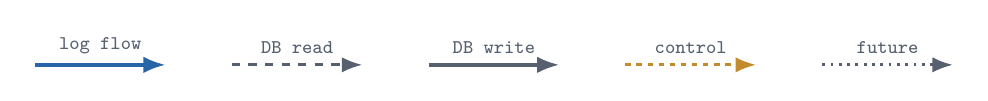
\begin{tikzpicture}
  \draw[logflow] (0,0) -- (1.8,0) node[midway,above,note] {log flow};
  \draw[dbread] (2.5,0) -- (4.3,0) node[midway,above,note] {DB read};
  \draw[dbwrite] (5.0,0) -- (6.8,0) node[midway,above,note] {DB write};
  \draw[control] (7.5,0) -- (9.3,0) node[midway,above,note] {control};
  \draw[futureline] (10.0,0) -- (11.8,0) node[midway,above,note] {future};
\end{tikzpicture}
\end{frame}

\section{1. Problem: OpenStack failures are hard to debug}

\begin{frame}{OpenStack Service Ecosystem}
\centering
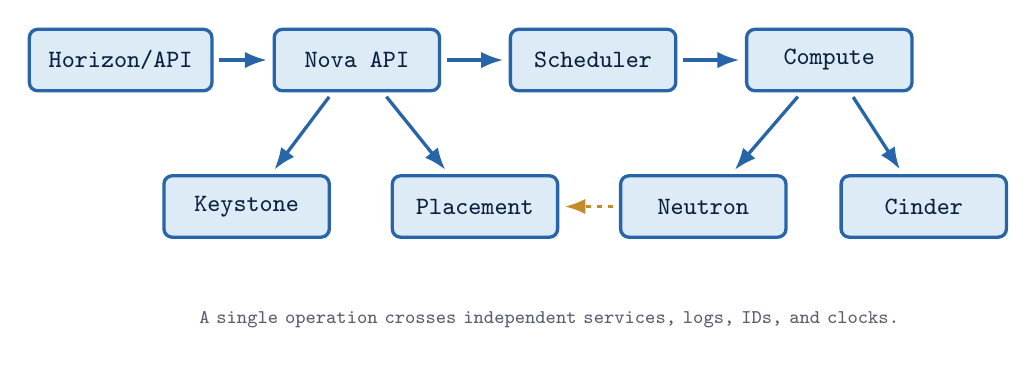
\begin{tikzpicture}[x=1cm,y=1.20cm]
  \node[svc,minimum width=2.1cm] (h) at (1,3.2) {Horizon/API};
  \node[svc,minimum width=2.1cm] (nova) at (4,3.2) {Nova API};
  \node[svc,minimum width=2.1cm] (sch) at (7,3.2) {Scheduler};
  \node[svc,minimum width=2.1cm] (comp) at (10,3.2) {Compute};
  \node[svc,minimum width=2.1cm] (key) at (2.6,1.65) {Keystone};
  \node[svc,minimum width=2.1cm] (place) at (5.5,1.65) {Placement};
  \node[svc,minimum width=2.1cm] (neut) at (8.4,1.65) {Neutron};
  \node[svc,minimum width=2.1cm] (cind) at (11.2,1.65) {Cinder};
  \draw[logflow] (h) -- (nova);
  \draw[logflow] (nova) -- (sch);
  \draw[logflow] (sch) -- (comp);
  \draw[logflow] (nova) -- (key);
  \draw[logflow] (nova) -- (place);
  \draw[logflow] (comp) -- (neut);
  \draw[logflow] (comp) -- (cind);
  \draw[control] (neut) -- (place);
  \node[note,text width=9cm] at (6.4,.45) {A single operation crosses independent services, logs, IDs, and clocks.};
\end{tikzpicture}
\end{frame}

\begin{frame}{Distributed Log Volume}
\centering
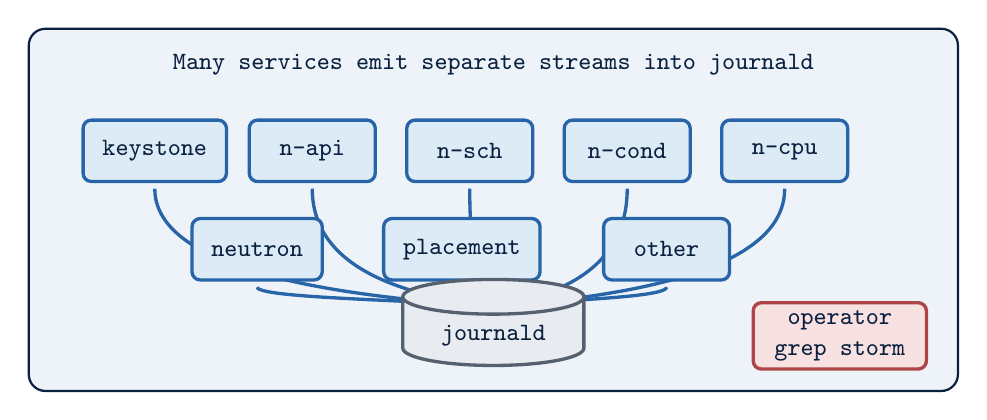
\begin{tikzpicture}[x=1cm,y=1cm]
  \node[zone,minimum width=11.8cm,minimum height=4.6cm] (z) at (6,2.25) {};
  \node[smalltitle] at (6,4.1) {Many services emit separate streams into journald};
  \foreach \n/\x/\y in {keystone/1.7/3,n-api/3.7/3,n-sch/5.7/3,n-cond/7.7/3,n-cpu/9.7/3,neutron/3/1.75,placement/5.6/1.75,other/8.2/1.75}{
    \node[svc,minimum width=1.6cm] (\n) at (\x,\y) {\n};
    \draw[logflow] (\n.south) .. controls (\x,1.1) and (6,1.1) .. (6,.65);
  }
  \node[db,minimum width=2.3cm] (j) at (6,.65) {journald};
  \node[err,minimum width=2.2cm] at (10.4,.65) {operator\\grep storm};
\end{tikzpicture}
\end{frame}

\begin{frame}{One Request Crosses Many Services}
\centering
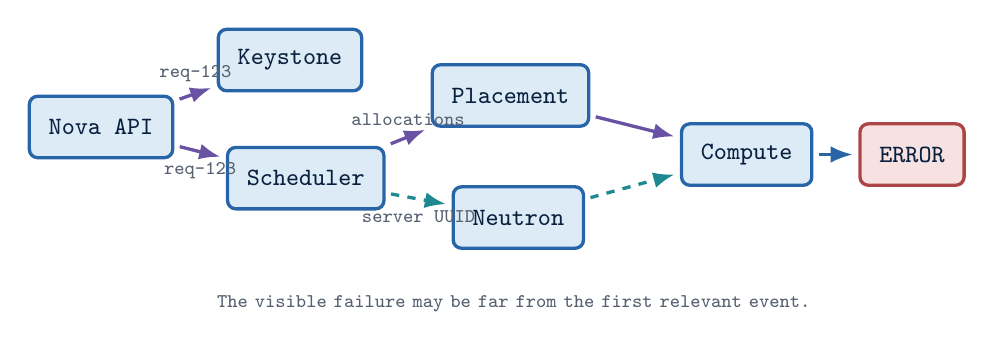
\begin{tikzpicture}[x=1cm,y=1cm]
  \node[svc] (api) at (1.2,2.8) {Nova API};
  \node[svc] (key) at (3.6,3.65) {Keystone};
  \node[svc] (sch) at (3.8,2.15) {Scheduler};
  \node[svc] (pl) at (6.4,3.2) {Placement};
  \node[svc] (neu) at (6.5,1.65) {Neutron};
  \node[svc] (cpu) at (9.4,2.45) {Compute};
  \node[err] (fail) at (11.5,2.45) {ERROR};
  \draw[edgeReq] (api) -- node[above,note] {req-123} (key);
  \draw[edgeReq] (api) -- node[below,note] {req-123} (sch);
  \draw[edgeReq] (sch) -- node[above,note] {allocations} (pl);
  \draw[edgeRes] (sch) -- node[below,note] {server UUID} (neu);
  \draw[edgeReq] (pl) -- (cpu);
  \draw[edgeRes] (neu) -- (cpu);
  \draw[logflow] (cpu) -- (fail);
  \node[note,text width=10cm] at (6.4,.55) {The visible failure may be far from the first relevant event.};
\end{tikzpicture}
\end{frame}

\begin{frame}{Why Isolated Log Inspection Fails}
\centering
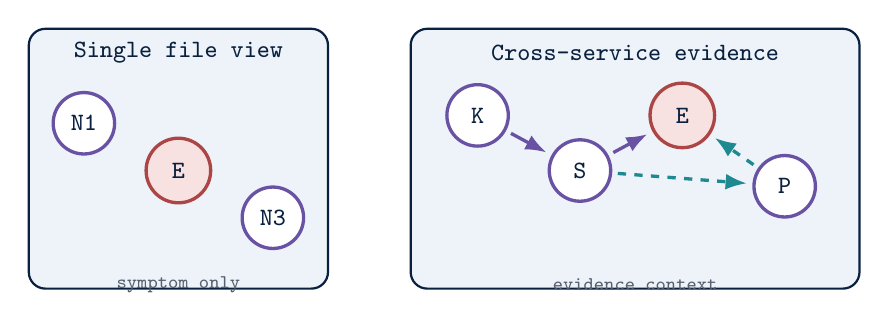
\begin{tikzpicture}[x=1cm,y=1cm]
  \node[zone,minimum width=3.8cm,minimum height=3.3cm] (left) at (2.7,2.35) {};
  \node[smalltitle] at (2.7,3.7) {Single file view};
  \node[event] at (1.5,2.8) {N1};
  \node[seed] at (2.7,2.2) {E};
  \node[event] at (3.9,1.6) {N3};
  \node[zone,minimum width=5.7cm,minimum height=3.3cm] (right) at (8.5,2.35) {};
  \node[smalltitle] at (8.5,3.7) {Cross-service evidence};
  \node[event] (a) at (6.5,2.9) {K};
  \node[event] (b) at (7.8,2.2) {S};
  \node[seed] (c) at (9.1,2.9) {E};
  \node[event] (d) at (10.4,2.0) {P};
  \draw[edgeReq] (a) -- (b);
  \draw[edgeReq] (b) -- (c);
  \draw[edgeRes] (b) -- (d);
  \draw[edgeRes] (d) -- (c);
  \node[note] at (2.7,.75) {symptom only};
  \node[note] at (8.5,.75) {evidence context};
\end{tikzpicture}
\end{frame}

\begin{frame}{Chronology Is Not Causality}
\centering
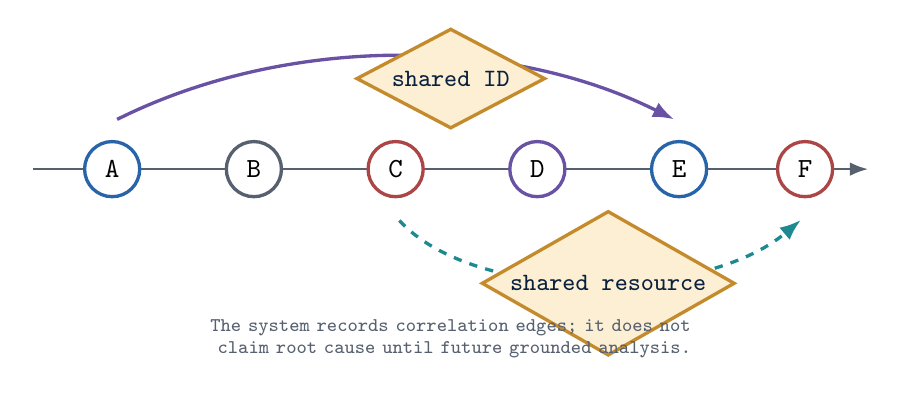
\begin{tikzpicture}[x=1cm,y=1cm]
  \draw[Slate,thick,-{Latex}] (1,2.5) -- (11.6,2.5);
  \foreach \x/\lab/\col in {2/A/MediumBlue,3.8/B/Slate,5.6/C/MutedRed,7.4/D/Purple,9.2/E/MediumBlue,10.8/F/MutedRed}{
    \node[circle,draw=\col,very thick,fill=white,minimum size=.7cm] at (\x,2.5) {\lab};
  }
  \draw[edgeReq] (2,3.1) .. controls (4.2,4.2) and (7.0,4.2) .. (9.2,3.1);
  \draw[edgeRes] (5.6,1.9) .. controls (6.6,.8) and (9.5,.8) .. (10.8,1.9);
  \node[warn,minimum width=2.4cm] at (6.3,3.65) {shared ID};
  \node[warn,minimum width=2.4cm] at (8.3,1.05) {shared resource};
  \node[note,text width=10.5cm] at (6.3,.35) {The system records correlation edges; it does not claim root cause until future grounded analysis.};
\end{tikzpicture}
\end{frame}

\begin{frame}{Monitoring vs Correlation vs RCA vs AI}
\centering
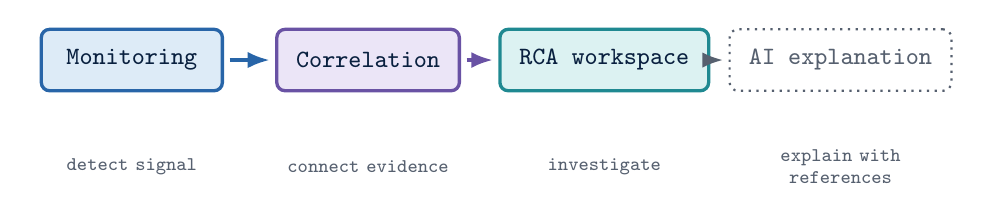
\begin{tikzpicture}[x=1cm,y=1cm]
  \node[svc,minimum width=2.3cm] (mon) at (1.5,2.7) {Monitoring};
  \node[graphlogic,minimum width=2.3cm] (corr) at (4.5,2.7) {Correlation};
  \node[transform,minimum width=2.3cm] (rca) at (7.5,2.7) {RCA workspace};
  \node[future,minimum width=2.3cm] (ai) at (10.5,2.7) {AI explanation};
  \draw[logflow] (mon) -- (corr);
  \draw[edgeReq] (corr) -- (rca);
  \draw[futureline] (rca) -- (ai);
  \node[note,text width=2.4cm] at (1.5,1.35) {detect signal};
  \node[note,text width=2.4cm] at (4.5,1.35) {connect evidence};
  \node[note,text width=2.4cm] at (7.5,1.35) {investigate};
  \node[note,text width=2.4cm] at (10.5,1.35) {explain with references};
\end{tikzpicture}
\end{frame}

\section{2. Goal: turn logs into investigation evidence}

\begin{frame}{Vision Architecture}
\centering
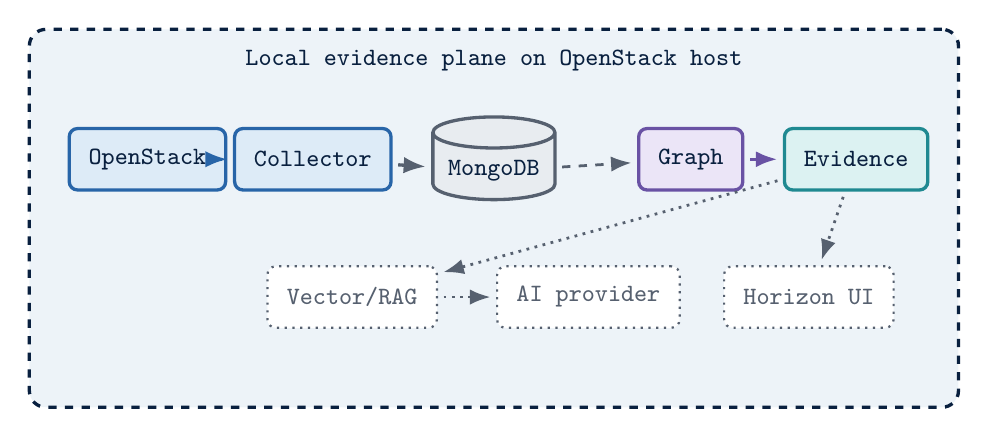
\begin{tikzpicture}[x=1cm,y=1cm]
  \node[machine,minimum width=11.8cm,minimum height=4.8cm] (mac) at (6,2.45) {};
  \node[smalltitle] at (6,4.45) {Local evidence plane on OpenStack host};
  \node[svc] (os) at (1.6,3.2) {OpenStack};
  \node[svc] (collector) at (3.7,3.2) {Collector};
  \node[db] (mongo) at (6,3.05) {MongoDB};
  \node[graphlogic] (graph) at (8.5,3.2) {Graph};
  \node[transform] (evidence) at (10.6,3.2) {Evidence};
  \node[future] (rag) at (4.2,1.45) {Vector/RAG};
  \node[future] (llm) at (7.2,1.45) {AI provider};
  \node[future] (ui) at (10,1.45) {Horizon UI};
  \draw[logflow] (os) -- (collector);
  \draw[dbwrite] (collector) -- (mongo);
  \draw[dbread] (mongo) -- (graph);
  \draw[edgeReq] (graph) -- (evidence);
  \draw[futureline] (evidence) -- (rag);
  \draw[futureline] (rag) -- (llm);
  \draw[futureline] (evidence) -- (ui);
\end{tikzpicture}
\end{frame}

\begin{frame}{Evidence-First Design}
\centering
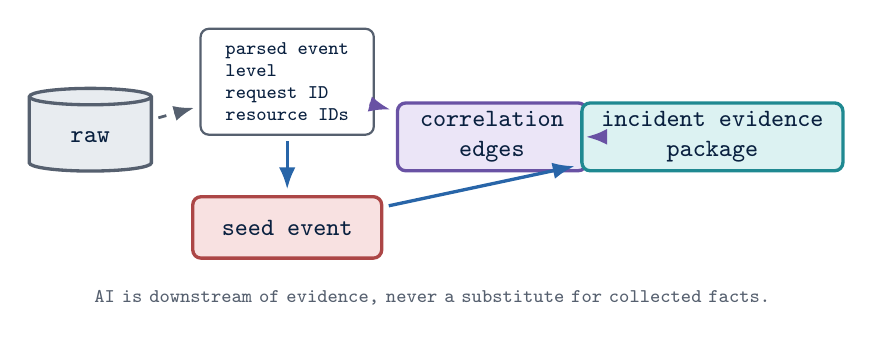
\begin{tikzpicture}[x=1cm,y=1cm]
  \node[db] (raw) at (1.7,2.5) {raw};
  \node[artifact,minimum width=2.2cm] (parsed) at (4.2,3.2) {parsed event\\level\\request ID\\resource IDs};
  \node[graphlogic,minimum width=2.4cm] (edges) at (6.8,2.5) {correlation\\edges};
  \node[err,minimum width=2.4cm] (seed) at (4.2,1.35) {seed event};
  \node[transform,minimum width=2.6cm] (inc) at (9.6,2.5) {incident evidence\\package};
  \draw[dbread] (raw) -- (parsed);
  \draw[edgeReq] (parsed) -- (edges);
  \draw[logflow] (parsed) -- (seed);
  \draw[edgeReq] (edges) -- (inc);
  \draw[logflow] (seed) -- (inc);
  \node[note,text width=9cm] at (6,.45) {AI is downstream of evidence, never a substitute for collected facts.};
\end{tikzpicture}
\end{frame}

\begin{frame}{Project Storyline}
\centering
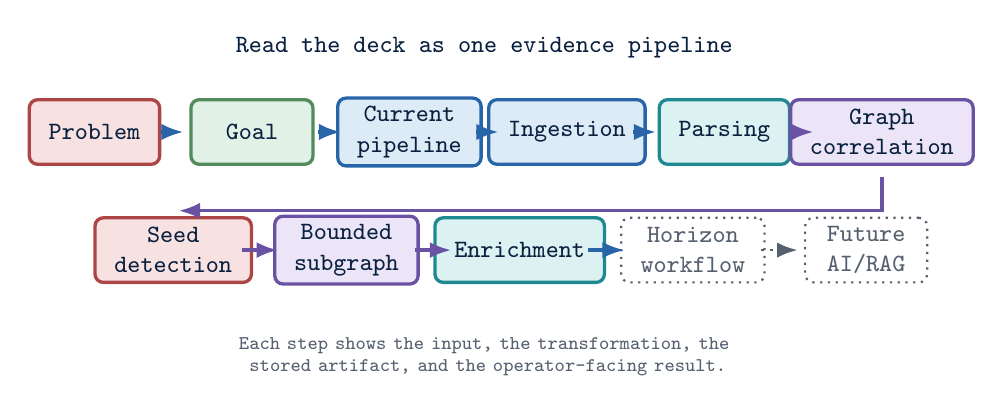
\begin{tikzpicture}[x=1cm,y=1cm]
  \node[smalltitle] at (6,4.62) {Read the deck as one evidence pipeline};
  \node[err,minimum width=1.55cm,minimum height=.82cm] at (1.05,3.55) {Problem};
  \node[ok,minimum width=1.55cm,minimum height=.82cm] at (3.05,3.55) {Goal};
  \node[svc,minimum width=1.55cm,minimum height=.82cm] at (5.05,3.55) {Current\\pipeline};
  \node[svc,minimum width=1.55cm,minimum height=.82cm] at (7.05,3.55) {Ingestion};
  \node[transform,minimum width=1.55cm,minimum height=.82cm] at (9.05,3.55) {Parsing};
  \node[graphlogic,minimum width=1.55cm,minimum height=.82cm] at (11.05,3.55) {Graph\\correlation};
  \node[err,minimum width=1.55cm,minimum height=.82cm] at (2.05,2.05) {Seed\\detection};
  \node[graphlogic,minimum width=1.55cm,minimum height=.82cm] at (4.25,2.05) {Bounded\\subgraph};
  \node[transform,minimum width=1.55cm,minimum height=.82cm] at (6.45,2.05) {Enrichment};
  \node[future,minimum width=1.55cm,minimum height=.82cm] at (8.65,2.05) {Horizon\\workflow};
  \node[future,minimum width=1.55cm,minimum height=.82cm] at (10.85,2.05) {Future\\AI/RAG};
  \draw[logflow] (1.82,3.55) -- (2.25,3.55);
  \draw[logflow] (3.82,3.55) -- (4.25,3.55);
  \draw[logflow] (5.82,3.55) -- (6.25,3.55);
  \draw[logflow] (7.82,3.55) -- (8.25,3.55);
  \draw[edgeReq] (9.82,3.55) -- (10.25,3.55);
  \draw[edgeReq] (11.05,3.05) |- (2.05,2.55);
  \draw[edgeReq] (2.85,2.05) -- (3.45,2.05);
  \draw[edgeReq] (5.05,2.05) -- (5.65,2.05);
  \draw[logflow] (7.25,2.05) -- (7.85,2.05);
  \draw[futureline] (9.45,2.05) -- (10.05,2.05);
  \node[note,text width=10.8cm] at (6,.7) {Each step shows the input, the transformation, the stored artifact, and the operator-facing result.};
\end{tikzpicture}
\end{frame}

\begin{frame}{Implemented vs Future System}
\centering
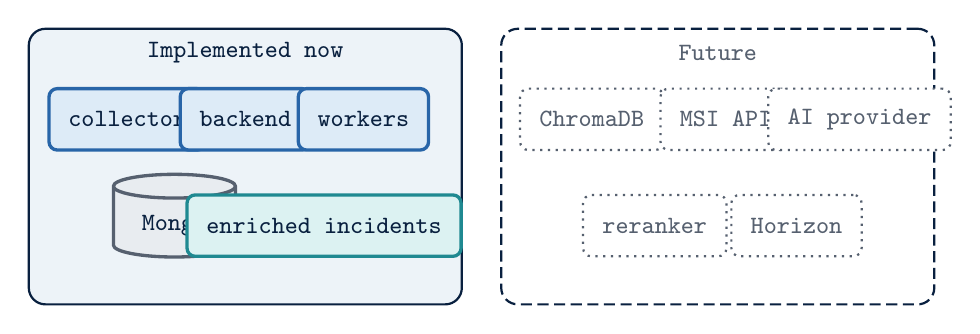
\begin{tikzpicture}[x=1cm,y=1cm]
  \node[zone,minimum width=5.5cm,minimum height=3.5cm] at (3.2,2.4) {};
  \node[smalltitle] at (3.2,3.85) {Implemented now};
  \node[svc] at (1.7,3.0) {collector};
  \node[svc] at (3.2,3.0) {backend};
  \node[worker] at (4.7,3.0) {workers};
  \node[db] at (2.3,1.65) {Mongo};
  \node[transform] at (4.2,1.65) {enriched incidents};
  \node[trust,minimum width=5.5cm,minimum height=3.5cm] at (9.2,2.4) {};
  \node[smalltitle,text=Slate] at (9.2,3.85) {Future};
  \node[future] at (7.6,3.0) {ChromaDB};
  \node[future] at (9.3,3.0) {MSI API};
  \node[future] at (11.0,3.0) {AI provider};
  \node[future] at (8.4,1.65) {reranker};
  \node[future] at (10.2,1.65) {Horizon};
\end{tikzpicture}
\end{frame}

\begin{frame}{Operator Interaction Model}
\centering
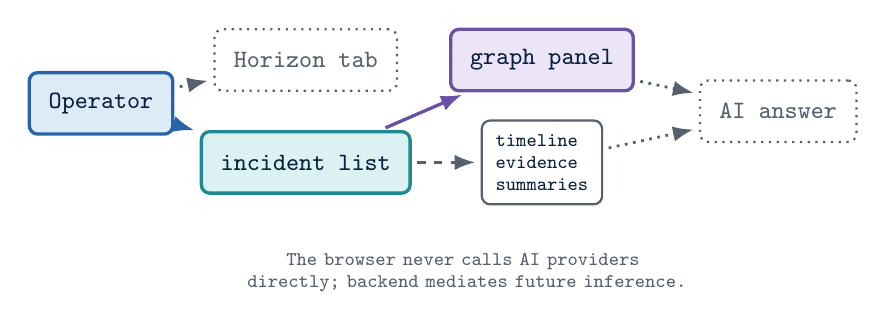
\begin{tikzpicture}[x=1cm,y=1cm]
  \node[svc] (op) at (1.4,2.7) {Operator};
  \node[future] (h) at (4.0,3.25) {Horizon tab};
  \node[transform] (inc) at (4.0,1.95) {incident list};
  \node[graphlogic] (g) at (7.0,3.25) {graph panel};
  \node[artifact] (ev) at (7.0,1.95) {timeline\\evidence\\summaries};
  \node[future] (ai) at (10.0,2.6) {AI answer};
  \draw[futureline] (op) -- (h);
  \draw[logflow] (op) -- (inc);
  \draw[edgeReq] (inc) -- (g);
  \draw[dbread] (inc) -- (ev);
  \draw[futureline] (g) -- (ai);
  \draw[futureline] (ev) -- (ai);
  \node[note,text width=8cm] at (6,.55) {The browser never calls AI providers directly; backend mediates future inference.};
\end{tikzpicture}
\end{frame}

\section{3. Current deployment topology}

\begin{frame}{Two-Machine Physical Topology}
\centering
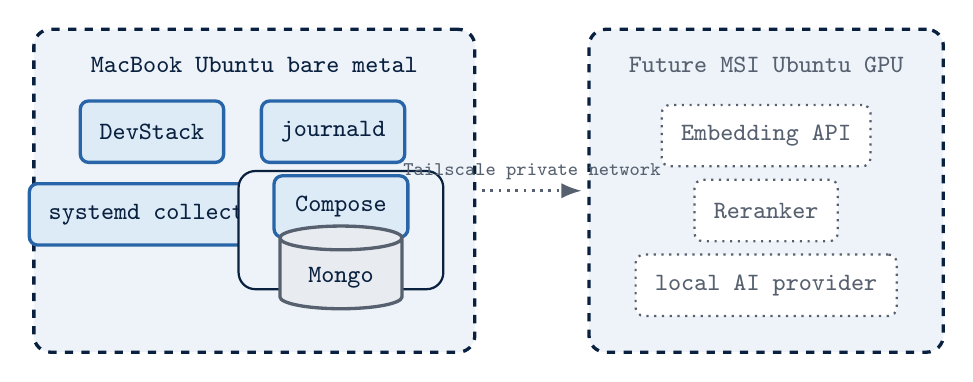
\begin{tikzpicture}[x=1cm,y=1cm]
  \node[machine,minimum width=5.6cm,minimum height=4.1cm] (mac) at (3.2,2.55) {};
  \node[smalltitle] at (3.2,4.15) {MacBook Ubuntu bare metal};
  \node[svc] at (1.9,3.3) {DevStack};
  \node[svc] at (4.2,3.3) {journald};
  \node[svc] at (2.0,2.25) {systemd collector};
  \node[zone,minimum width=2.6cm,minimum height=1.5cm] at (4.3,2.05) {};
  \node[svc,minimum width=1.7cm] at (4.3,2.35) {Compose};
  \node[db] at (4.3,1.45) {Mongo};
  \node[machine,minimum width=4.5cm,minimum height=4.1cm] (msi) at (9.7,2.55) {};
  \node[smalltitle,text=Slate] at (9.7,4.15) {Future MSI Ubuntu GPU};
  \node[future] at (9.7,3.25) {Embedding API};
  \node[future] at (9.7,2.3) {Reranker};
  \node[future] at (9.7,1.35) {local AI provider};
  \draw[futureline] (mac) -- node[above,note] {Tailscale private network} (msi);
\end{tikzpicture}
\end{frame}

\begin{frame}{MacBook Host and Container Boundaries}
\centering
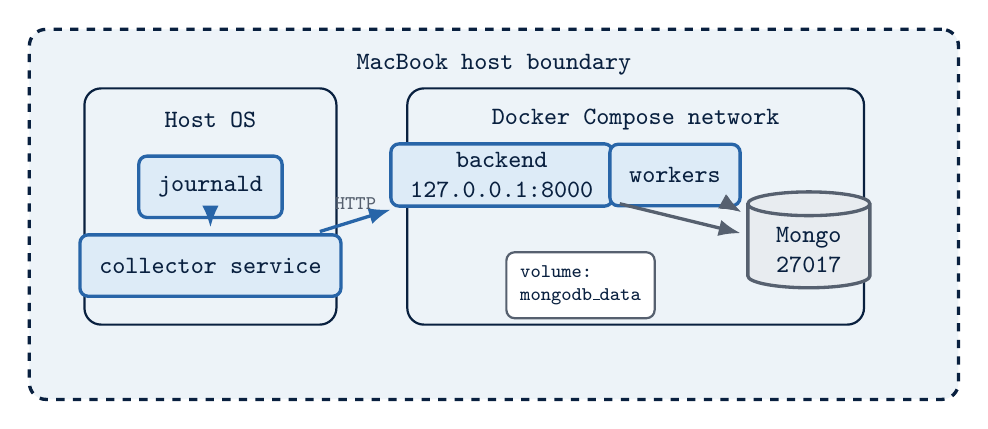
\begin{tikzpicture}[x=1cm,y=1cm]
  \node[machine,minimum width=11.8cm,minimum height=4.7cm] at (6,2.45) {};
  \node[smalltitle] at (6,4.35) {MacBook host boundary};
  \node[zone,minimum width=3.2cm,minimum height=3.0cm] at (2.4,2.55) {};
  \node[smalltitle] at (2.4,3.65) {Host OS};
  \node[svc] (journal) at (2.4,2.8) {journald};
  \node[svc] (collector) at (2.4,1.8) {collector service};
  \node[zone,minimum width=5.8cm,minimum height=3.0cm] at (7.8,2.55) {};
  \node[smalltitle] at (7.8,3.65) {Docker Compose network};
  \node[svc] (backend) at (6.1,2.95) {backend\\127.0.0.1:8000};
  \node[worker] (workers) at (8.3,2.95) {workers};
  \node[db] (mongo) at (10.0,2.0) {Mongo\\27017};
  \node[artifact] at (7.1,1.55) {volume:\\mongodb\_data};
  \draw[logflow] (journal) -- (collector);
  \draw[logflow] (collector) -- node[above,note] {HTTP} (backend);
  \draw[dbwrite] (backend) -- (mongo);
  \draw[dbread] (workers) -- (mongo);
  \draw[dbwrite] (workers) -- (mongo);
\end{tikzpicture}
\end{frame}

\begin{frame}{Ports, Protocols, and Trust Boundaries}
\centering
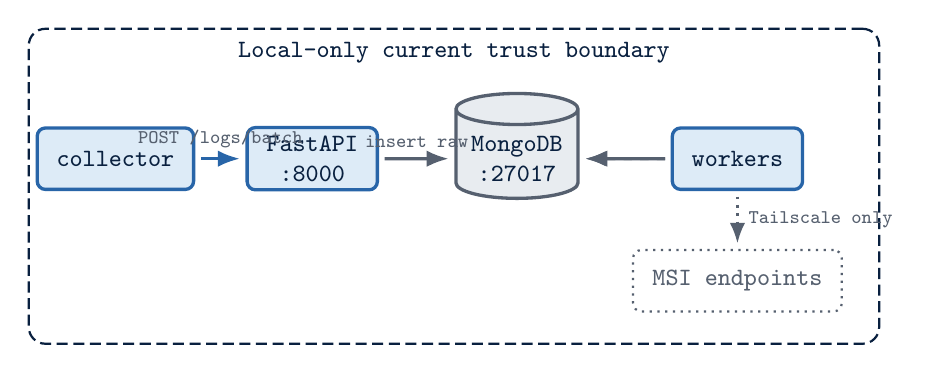
\begin{tikzpicture}[x=1cm,y=1cm]
  \node[trust,minimum width=10.8cm,minimum height=4.0cm] at (6,2.45) {};
  \node[smalltitle] at (6,4.15) {Local-only current trust boundary};
  \node[svc] (col) at (1.7,2.8) {collector};
  \node[svc] (api) at (4.2,2.8) {FastAPI\\:8000};
  \node[db] (mongo) at (6.8,2.8) {MongoDB\\:27017};
  \node[worker] (w) at (9.6,2.8) {workers};
  \node[future] (msi) at (9.6,1.25) {MSI endpoints};
  \draw[logflow] (col) -- node[above,note] {POST /logs/batch} (api);
  \draw[dbwrite] (api) -- node[above,note] {insert raw} (mongo);
  \draw[dbread] (w) -- (mongo);
  \draw[dbwrite] (w) -- (mongo);
  \draw[futureline] (w) -- node[right,note] {Tailscale only} (msi);
\end{tikzpicture}
\end{frame}

\section{4. Current implemented pipeline}

\begin{frame}{Runtime Dependency Graph}
\centering
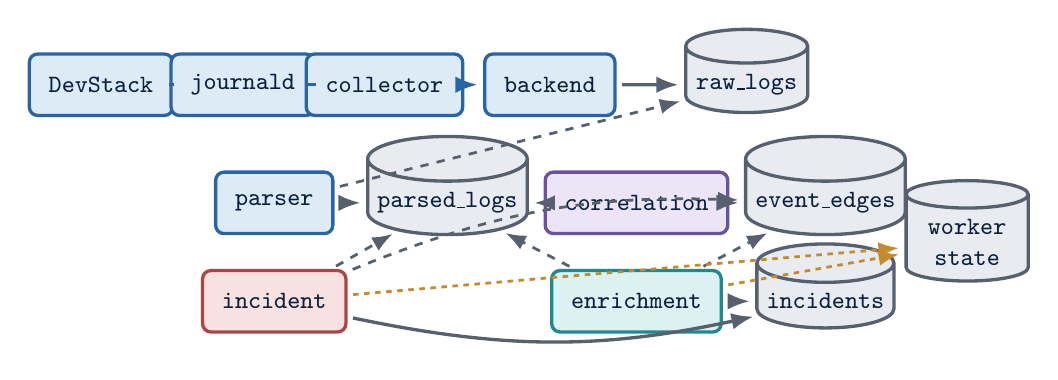
\begin{tikzpicture}[x=1cm,y=1cm]
  \node[svc] (dev) at (1,3.2) {DevStack};
  \node[svc] (j) at (2.8,3.2) {journald};
  \node[svc] (c) at (4.6,3.2) {collector};
  \node[svc] (api) at (6.7,3.2) {backend};
  \node[db] (raw) at (9.2,3.2) {raw\_logs};
  \node[worker] (p) at (3.2,1.7) {parser};
  \node[db] (parsed) at (5.4,1.7) {parsed\_logs};
  \node[graphlogic] (corr) at (7.8,1.7) {correlation};
  \node[db] (edges) at (10.2,1.7) {event\_edges};
  \node[err] (incw) at (3.2,.45) {incident};
  \node[transform] (enw) at (7.8,.45) {enrichment};
  \node[db] (incs) at (10.2,.45) {incidents};
  \node[db] (state) at (12.0,1.2) {worker\\state};
  \draw[logflow] (dev)--(j)--(c)--(api);
  \draw[dbwrite] (api)--(raw);
  \draw[dbread] (p) -- (raw);
  \draw[dbwrite] (p) -- (parsed);
  \draw[dbread] (corr) -- (parsed);
  \draw[dbwrite] (corr) -- (edges);
  \draw[dbread] (incw) -- (parsed);
  \draw[dbread] (incw) to[bend left=12] (edges);
  \draw[dbwrite] (incw) to[bend right=12] (incs);
  \draw[dbread] (enw) -- (parsed);
  \draw[dbread] (enw) -- (edges);
  \draw[dbwrite] (enw) -- (incs);
  \draw[control] (incw) -- (state);
  \draw[control] (enw) -- (state);
\end{tikzpicture}
\end{frame}

\begin{frame}{Future Runtime Extensions}
\centering
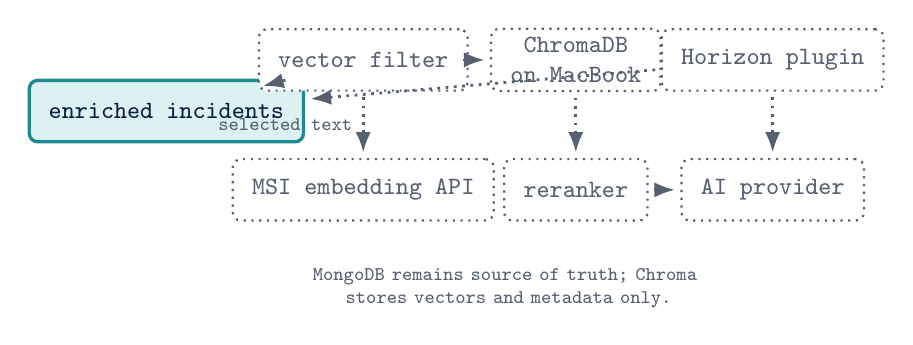
\begin{tikzpicture}[x=1cm,y=1cm]
  \node[transform] (inc) at (1.7,2.8) {enriched incidents};
  \node[future] (filter) at (4.2,3.45) {vector filter};
  \node[future] (chroma) at (6.9,3.45) {ChromaDB\\on MacBook};
  \node[future] (emb) at (4.2,1.8) {MSI embedding API};
  \node[future] (rerank) at (6.9,1.8) {reranker};
  \node[future] (ollama) at (9.4,1.8) {AI provider};
  \node[future] (h) at (9.4,3.45) {Horizon plugin};
  \draw[futureline] (inc) -- (filter);
  \draw[futureline] (filter) -- (chroma);
  \draw[futureline] (filter) -- node[left,note] {selected text} (emb);
  \draw[futureline] (chroma) -- (rerank);
  \draw[futureline] (rerank) -- (ollama);
  \draw[futureline] (h) -- (inc);
  \draw[futureline] (h) -- (ollama);
  \node[note,text width=9cm] at (6,.55) {MongoDB remains source of truth; Chroma stores vectors and metadata only.};
\end{tikzpicture}
\end{frame}

\section{5. Evidence lineage and transformations}

\begin{frame}{Data Lineage Map}
\centering
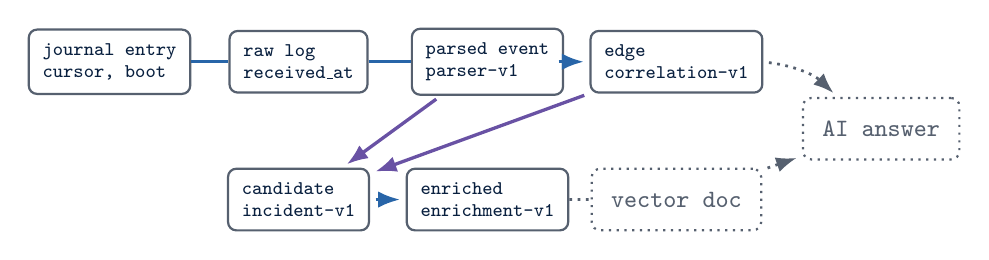
\begin{tikzpicture}[x=1cm,y=1cm]
  \node[artifact] (j) at (1,3.2) {journal entry\\cursor, boot};
  \node[artifact] (raw) at (3.4,3.2) {raw log\\received\_at};
  \node[artifact] (parsed) at (5.8,3.2) {parsed event\\parser-v1};
  \node[artifact] (edge) at (8.2,3.2) {edge\\correlation-v1};
  \node[artifact] (cand) at (3.4,1.45) {candidate\\incident-v1};
  \node[artifact] (en) at (5.8,1.45) {enriched\\enrichment-v1};
  \node[future] (vec) at (8.2,1.45) {vector doc};
  \node[future] (ans) at (10.8,2.35) {AI answer};
  \draw[logflow] (j)--(raw)--(parsed)--(edge);
  \draw[edgeReq] (parsed) -- (cand);
  \draw[edgeReq] (edge) -- (cand);
  \draw[logflow] (cand)--(en);
  \draw[futureline] (en)--(vec)--(ans);
  \draw[futureline] (edge) to[bend left=18] (ans);
\end{tikzpicture}
\end{frame}

\begin{frame}{Parsing and Graph Relationships}
\centering
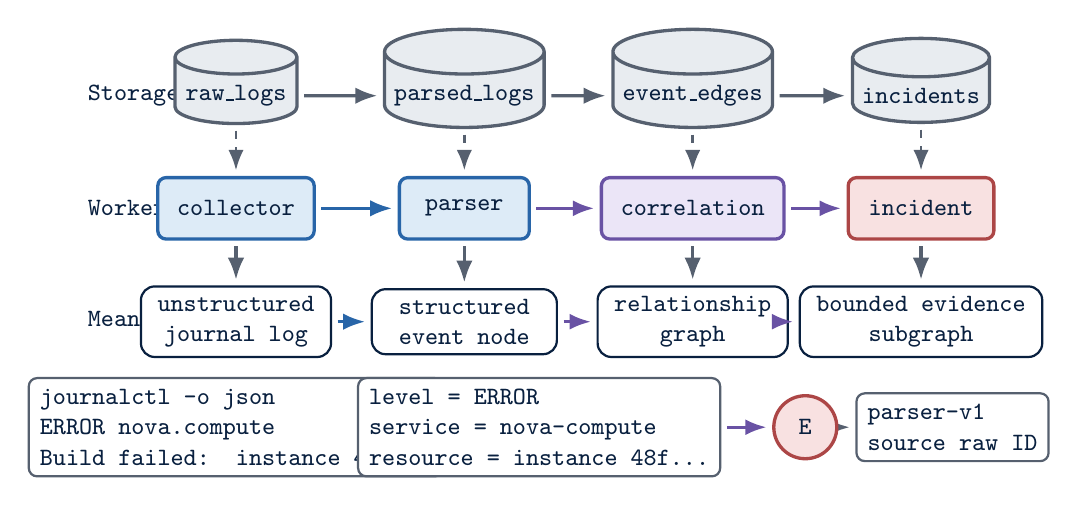
\begin{tikzpicture}[x=1cm,y=1cm]
  \node[bandlabel] at (.85,5.05) {Storage};
  \node[db,minimum width=1.55cm] (rawdb) at (2.15,5.05) {raw\_logs};
  \node[db,minimum width=1.72cm] (parseddb) at (5.05,5.05) {parsed\_logs};
  \node[db,minimum width=1.72cm] (edgedb) at (7.95,5.05) {event\_edges};
  \node[db,minimum width=1.55cm] (incdb) at (10.85,5.05) {incidents};
  \draw[dbwrite] (rawdb) -- (parseddb);
  \draw[dbwrite] (parseddb) -- (edgedb);
  \draw[dbwrite] (edgedb) -- (incdb);

  \node[bandlabel] at (.85,3.62) {Workers};
  \node[worker,minimum width=1.65cm] (collector) at (2.15,3.62) {collector};
  \node[worker,minimum width=1.65cm] (parser) at (5.05,3.62) {parser};
  \node[graphlogic,minimum width=1.85cm] (corr) at (7.95,3.62) {correlation};
  \node[err,minimum width=1.85cm] (incident) at (10.85,3.62) {incident};
  \draw[logflow] (collector) -- (parser);
  \draw[edgeReq] (parser) -- (corr);
  \draw[edgeReq] (corr) -- (incident);

  \node[bandlabel] at (.85,2.18) {Meaning};
  \node[pipelinebox,minimum width=2.35cm] (raw) at (2.15,2.18) {unstructured\\journal log};
  \node[pipelinebox,minimum width=2.35cm] (parsed) at (5.05,2.18) {structured\\event node};
  \node[pipelinebox,minimum width=2.35cm] (edges) at (7.95,2.18) {relationship\\graph};
  \node[pipelinebox,minimum width=2.35cm] (package) at (10.85,2.18) {bounded evidence\\subgraph};
  \draw[logflow] (raw) -- (parsed);
  \draw[edgeReq] (parsed) -- (edges);
  \draw[edgeReq] (edges) -- (package);

  \draw[dbread] (rawdb) -- (collector);
  \draw[dbread] (parseddb) -- (parser);
  \draw[dbread] (edgedb) -- (corr);
  \draw[dbread] (incdb) -- (incident);
  \draw[dbwrite] (collector) -- (raw);
  \draw[dbwrite] (parser) -- (parsed);
  \draw[dbwrite] (corr) -- (edges);
  \draw[dbwrite] (incident) -- (package);

  \node[miniartifact,minimum width=3.25cm] (example) at (2.15,.84) {journalctl -o json\\ERROR nova.compute\\Build failed: instance 48f...};
  \node[miniartifact,minimum width=3.28cm] (fields) at (6.00,.84) {level = ERROR\\service = nova-compute\\resource = instance 48f...};
  \node[eventErr] (n1) at (9.38,.84) {E};
  \node[miniartifact,minimum width=1.95cm] (version) at (11.25,.84) {parser-v1\\source raw ID};
  \begin{scope}[on background layer]
    \draw[logflow] (example.east) -- (fields.west);
    \draw[edgeReq] (fields.east) -- (n1.west);
    \draw[dbwrite] (n1.east) -- (version.west);
  \end{scope}
\end{tikzpicture}
\end{frame}

\begin{frame}{Correlation: Structured Events to Graph Edges}
\centering
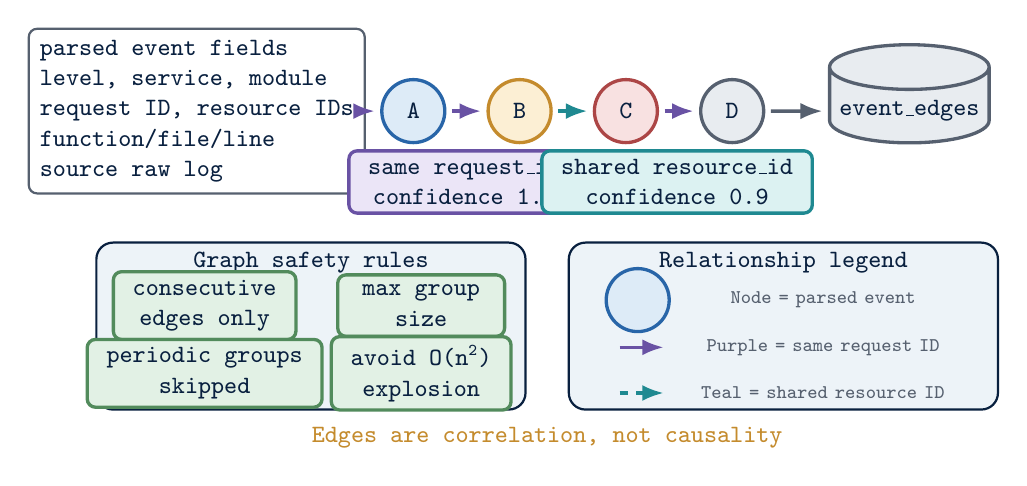
\begin{tikzpicture}[x=1cm,y=1cm]
  \node[miniartifact,minimum width=3.25cm] (fields) at (1.95,4.35) {parsed event fields\\level, service, module\\request ID, resource IDs\\function/file/line\\source raw log};
  \node[eventInfo] (a) at (4.70,4.35) {A};
  \node[eventWarn] (b) at (6.05,4.35) {B};
  \node[eventErr] (c) at (7.40,4.35) {C};
  \node[eventDebug] (d) at (8.75,4.35) {D};
  \node[db] (edgedb2) at (11.00,4.35) {event\_edges};
  \draw[edgeReq] (fields) -- (a);
  \draw[edgeReq] (a) -- (b);
  \draw[edgeRes] (b) -- (c);
  \draw[edgeReq] (c) -- (d);
  \draw[dbwrite] (d) -- (edgedb2);
  \node[graphlogic,minimum width=2.45cm,minimum height=.62cm] at (5.35,3.45) {same request\_id\\confidence 1.0};
  \node[transform,minimum width=2.45cm,minimum height=.62cm] at (8.05,3.45) {shared resource\_id\\confidence 0.9};

  \node[zone,minimum width=5.45cm,minimum height=2.12cm] at (3.40,1.62) {};
  \node[smalltitle] at (3.40,2.43) {Graph safety rules};
  \node[ok,minimum width=2.12cm] at (2.05,1.88) {consecutive\\edges only};
  \node[ok,minimum width=2.12cm] at (4.80,1.88) {max group\\size};
  \node[ok,minimum width=2.12cm] at (2.05,1.02) {periodic groups\\skipped};
  \node[ok,minimum width=2.12cm] at (4.80,1.02) {avoid O(n\textsuperscript{2})\\explosion};

  \node[zone,minimum width=5.45cm,minimum height=2.12cm] at (9.40,1.62) {};
  \node[smalltitle] at (9.40,2.43) {Relationship legend};
  \node[eventInfo] at (7.55,1.95) {};
  \node[note,anchor=west,text width=3.45cm] at (8.05,1.95) {Node = parsed event};
  \draw[edgeReq] (7.25,1.35) -- (7.95,1.35);
  \node[note,anchor=west,text width=3.45cm] at (8.05,1.35) {Purple = same request ID};
  \draw[edgeRes] (7.25,.77) -- (7.95,.77);
  \node[note,anchor=west,text width=3.45cm] at (8.05,.77) {Teal = shared resource ID};

  \node[font=\bfseries\small,text=Amber,align=center] at (6.40,.20) {Edges are correlation, not causality};
\end{tikzpicture}
\end{frame}

\begin{frame}{Incident Evidence Package}
\centering
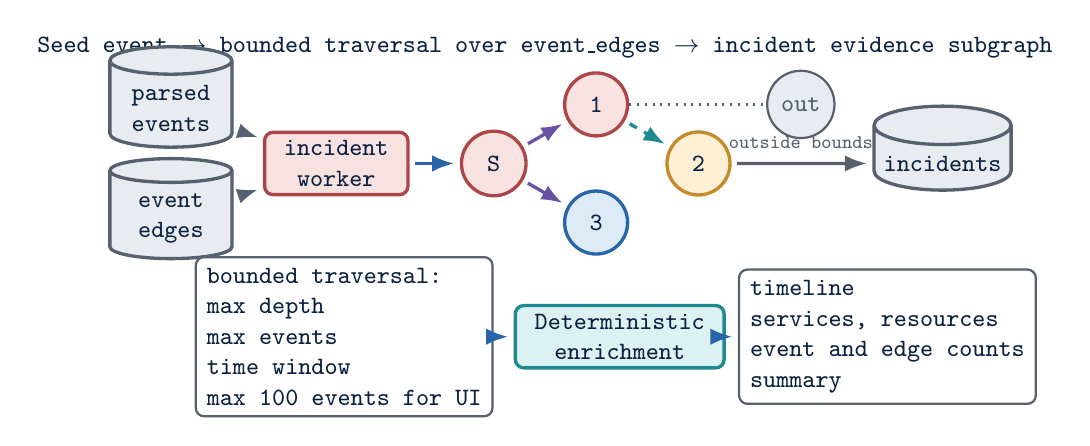
\begin{tikzpicture}[x=1cm,y=1cm]
  \node[smalltitle] at (6,5.02) {Seed event $\rightarrow$ bounded traversal over event\_edges $\rightarrow$ incident evidence subgraph};
  \node[db] (parsed3) at (1.25,4.25) {parsed\\events};
  \node[db] (edges3) at (1.25,2.85) {event\\edges};
  \node[err,minimum width=1.75cm] (worker3) at (3.35,3.55) {incident\\worker};
  \node[seed] (seed3) at (5.35,3.55) {S};
  \node[eventErr] (e1) at (6.65,4.30) {1};
  \node[eventWarn] (e2) at (7.95,3.55) {2};
  \node[eventInfo] (e3) at (6.65,2.80) {3};
  \node[excluded] (out) at (9.25,4.30) {out};
  \node[db] (incidents3) at (11.05,3.55) {incidents};
  \draw[dbread] (parsed3) -- (worker3);
  \draw[dbread] (edges3) -- (worker3);
  \draw[logflow] (worker3) -- (seed3);
  \draw[edgeReq] (seed3) -- (e1);
  \draw[edgeRes] (e1) -- (e2);
  \draw[edgeReq] (seed3) -- (e3);
  \draw[Slate,dotted,thick] (e1) -- (out);
  \node[note] at (9.25,3.82) {outside bounds};
  \draw[dbwrite] (e2) -- (incidents3);

  \node[miniartifact,minimum width=3.05cm] (bounds3) at (3.45,1.35) {bounded traversal:\\max depth\\max events\\time window\\max 100 events for UI};
  \node[transform,minimum width=2.30cm] (enrich3) at (6.95,1.35) {Deterministic\\enrichment};
  \node[miniartifact,minimum width=3.15cm] (summary3) at (10.35,1.35) {timeline\\services, resources\\event and edge counts\\summary};
  \draw[logflow] (bounds3.east) -- (enrich3.west);
  \draw[logflow] (enrich3.east) -- (summary3.west);

\end{tikzpicture}
\end{frame}

\begin{frame}{Artifact Responsibilities}
\centering
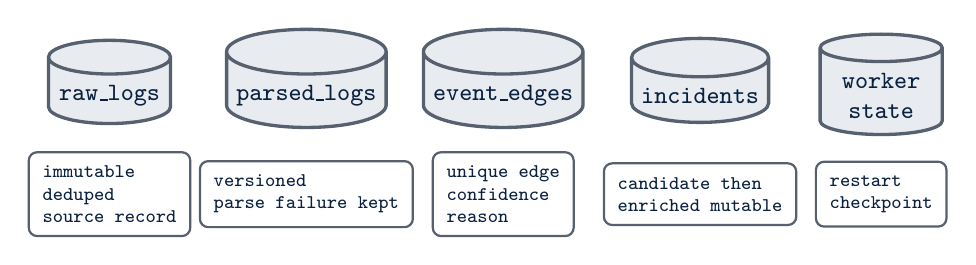
\begin{tikzpicture}[x=1cm,y=1cm]
  \node[db] (raw) at (1.5,2.7) {raw\_logs};
  \node[artifact] at (1.5,1.45) {immutable\\deduped\\source record};
  \node[db] (parsed) at (4,2.7) {parsed\_logs};
  \node[artifact] at (4,1.45) {versioned\\parse failure kept};
  \node[db] (edges) at (6.5,2.7) {event\_edges};
  \node[artifact] at (6.5,1.45) {unique edge\\confidence\\reason};
  \node[db] (inc) at (9,2.7) {incidents};
  \node[artifact] at (9,1.45) {candidate then\\enriched mutable};
  \node[db] (state) at (11.3,2.7) {worker\\state};
  \node[artifact] at (11.3,1.45) {restart\\checkpoint};
\end{tikzpicture}
\end{frame}

\section{6. Log ingestion: journald to MongoDB}

\begin{frame}{Monitored DevStack Units}
\centering
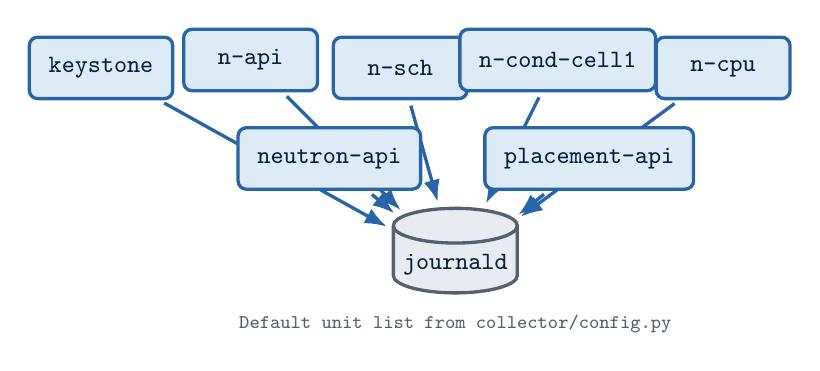
\begin{tikzpicture}[x=1cm,y=1cm]
  \node[db] (j) at (6,1) {journald};
  \foreach \name/\x/\y in {keystone/1.5/3.5,n-api/3.4/3.6,n-sch/5.3/3.5,n-cond-cell1/7.3/3.6,n-cpu/9.4/3.5,neutron-api/4.4/2.35,placement-api/7.7/2.35}{
    \node[svc,minimum width=1.7cm] (\name) at (\x,\y) {\name};
    \draw[logflow] (\name) -- (j);
  }
  \node[note] at (6,.25) {Default unit list from collector/config.py};
\end{tikzpicture}
\end{frame}

\begin{frame}{Collector Sequence: Cursor Advances After ACK}
\centering
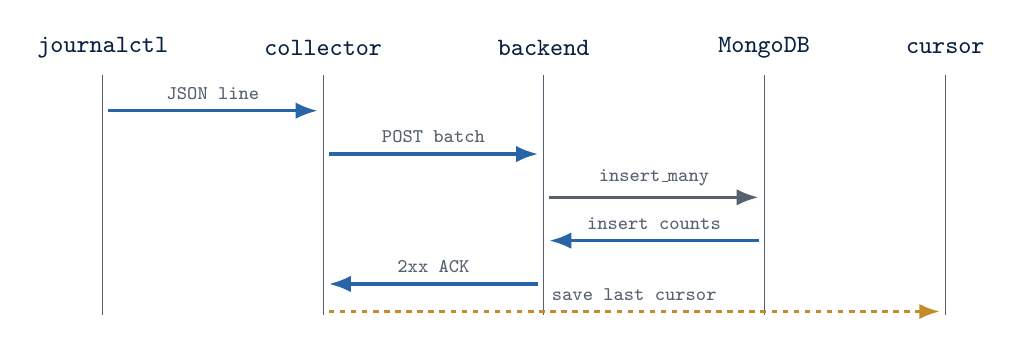
\begin{tikzpicture}[x=1cm,y=1cm]
  \foreach \name/\x in {journalctl/1.4,collector/4.2,backend/7.0,MongoDB/9.8,cursor/12.1}{
    \node[smalltitle] at (\x,4.1) {\name};
    \draw[Slate,thin] (\x,3.75) -- (\x,.7);
  }
  \draw[logflow] (1.4,3.3) -- node[above,note] {JSON line} (4.2,3.3);
  \draw[logflow] (4.2,2.75) -- node[above,note] {POST batch} (7.0,2.75);
  \draw[dbwrite] (7.0,2.2) -- node[above,note] {insert\_many} (9.8,2.2);
  \draw[logflow] (9.8,1.65) -- node[above,note] {insert counts} (7.0,1.65);
  \draw[logflow] (7.0,1.1) -- node[above,note] {2xx ACK} (4.2,1.1);
  \draw[control] (4.2,.75) -- node[above,note] {save last cursor} (12.1,.75);
\end{tikzpicture}
\end{frame}

\begin{frame}{Collector State Machine}
\centering
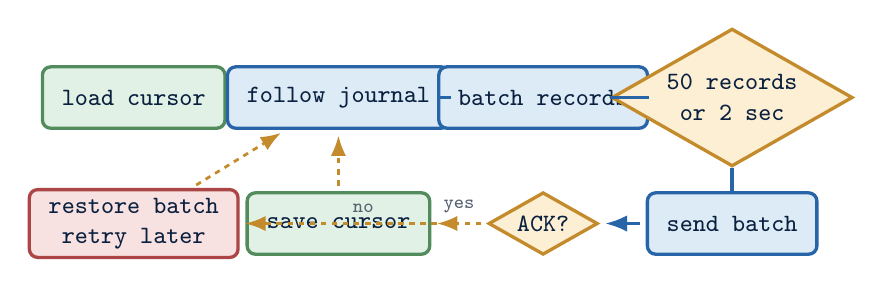
\begin{tikzpicture}[x=1cm,y=1cm]
  \node[ok] (load) at (1.4,3) {load cursor};
  \node[svc] (follow) at (4.0,3) {follow journal};
  \node[svc] (batch) at (6.6,3) {batch records};
  \node[warn] (flush) at (9.0,3) {50 records\\or 2 sec};
  \node[svc] (send) at (9.0,1.4) {send batch};
  \node[warn] (ack) at (6.6,1.4) {ACK?};
  \node[ok] (save) at (4.0,1.4) {save cursor};
  \node[err] (restore) at (1.4,1.4) {restore batch\\retry later};
  \draw[logflow] (load)--(follow)--(batch)--(flush)--(send)--(ack);
  \draw[control] (ack)--node[above,note]{yes}(save);
  \draw[control] (save)--(follow);
  \draw[control] (ack)--node[above,note]{no}(restore);
  \draw[control] (restore)--(follow);
\end{tikzpicture}
\end{frame}

\begin{frame}{Backend Unavailable: Retry Branch}
\centering
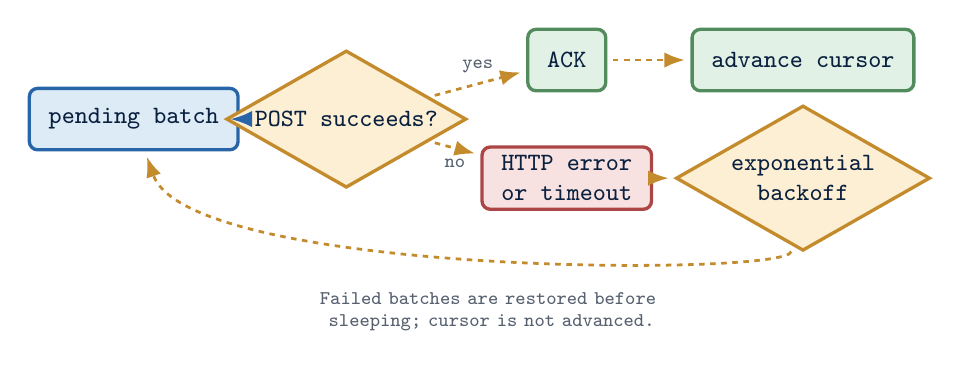
\begin{tikzpicture}[x=1cm,y=1cm]
  \node[svc] (batch) at (1.5,2.8) {pending batch};
  \node[warn] (post) at (4.2,2.8) {POST succeeds?};
  \node[ok] (ack) at (7,3.55) {ACK};
  \node[err] (fail) at (7,2.05) {HTTP error\\or timeout};
  \node[warn] (backoff) at (10,2.05) {exponential\\backoff};
  \node[ok] (cursor) at (10,3.55) {advance cursor};
  \draw[logflow] (batch)--(post);
  \draw[control] (post)--node[above,note]{yes}(ack);
  \draw[control] (ack)--(cursor);
  \draw[control] (post)--node[below,note]{no}(fail);
  \draw[control] (fail)--(backoff);
  \draw[control] (backoff) .. controls (9.8,.8) and (2.2,.8) .. (batch);
  \node[note,text width=8cm] at (6,.35) {Failed batches are restored before sleeping; cursor is not advanced.};
\end{tikzpicture}
\end{frame}

\begin{frame}{Crash Recovery and Duplicate Prevention}
\centering
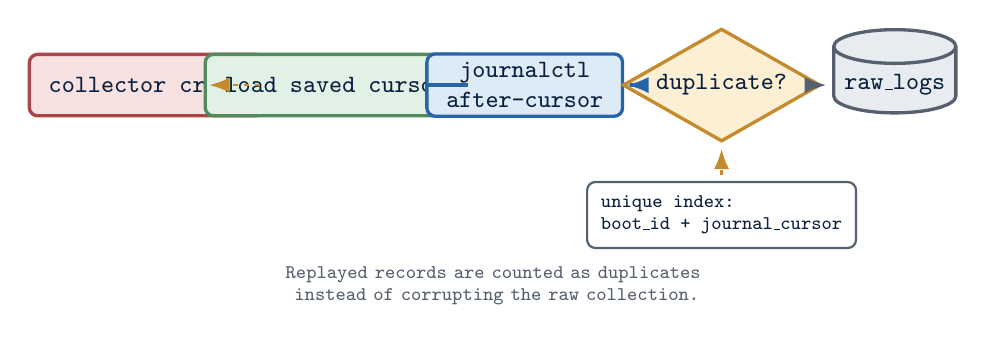
\begin{tikzpicture}[x=1cm,y=1cm]
  \node[err] (crash) at (1.6,3) {collector crash};
  \node[ok] (load) at (4.0,3) {load saved cursor};
  \node[svc] (replay) at (6.4,3) {journalctl\\after-cursor};
  \node[warn] (dup) at (8.9,3) {duplicate?};
  \node[db] (raw) at (11.1,3) {raw\_logs};
  \node[artifact] (idx) at (8.9,1.35) {unique index:\\boot\_id + journal\_cursor};
  \draw[control] (crash)--(load);
  \draw[logflow] (load)--(replay)--(dup);
  \draw[dbwrite] (dup)--(raw);
  \draw[control] (idx)--(dup);
  \node[note,text width=8cm] at (6,.45) {Replayed records are counted as duplicates instead of corrupting the raw collection.};
\end{tikzpicture}
\end{frame}

\section{7. Raw evidence storage}

\begin{frame}{raw\_logs Schema as Evidence Envelope}
\centering
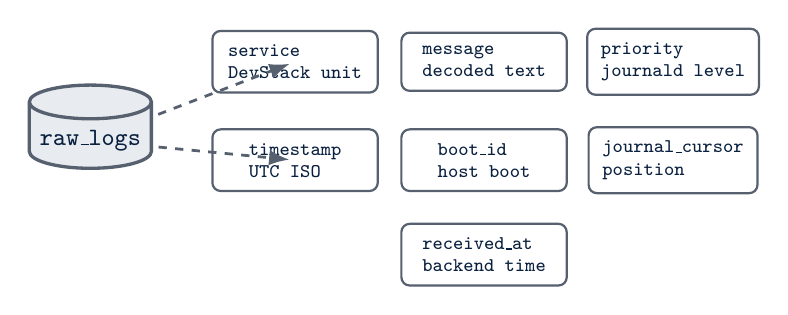
\begin{tikzpicture}[x=1cm,y=1cm]
  \node[db] (raw) at (1.4,2.5) {raw\_logs};
  \node[artifact,minimum width=2.1cm] at (4.0,3.5) {service\\DevStack unit};
  \node[artifact,minimum width=2.1cm] at (6.4,3.5) {message\\decoded text};
  \node[artifact,minimum width=2.1cm] at (8.8,3.5) {priority\\journald level};
  \node[artifact,minimum width=2.1cm] at (4.0,2.25) {timestamp\\UTC ISO};
  \node[artifact,minimum width=2.1cm] at (6.4,2.25) {boot\_id\\host boot};
  \node[artifact,minimum width=2.1cm] at (8.8,2.25) {journal\_cursor\\position};
  \node[artifact,minimum width=2.1cm] at (6.4,1.05) {received\_at\\backend time};
  \draw[dbread] (raw) -- (4.0,3.5);
  \draw[dbread] (raw) -- (4.0,2.25);
\end{tikzpicture}
\end{frame}

\begin{frame}{boot\_id + journal\_cursor Identity}
\centering
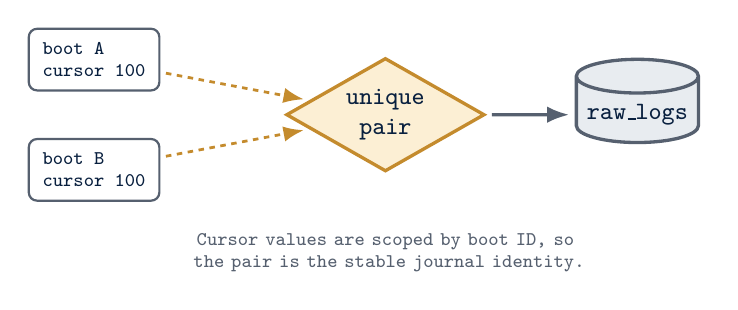
\begin{tikzpicture}[x=1cm,y=1cm]
  \node[artifact] (a) at (2.3,3.2) {boot A\\cursor 100};
  \node[artifact] (b) at (2.3,1.8) {boot B\\cursor 100};
  \node[warn] (idx) at (6.0,2.5) {unique\\pair};
  \node[db] (raw) at (9.2,2.5) {raw\_logs};
  \draw[control] (a)--(idx);
  \draw[control] (b)--(idx);
  \draw[dbwrite] (idx)--(raw);
  \node[note,text width=8cm] at (6,.75) {Cursor values are scoped by boot ID, so the pair is the stable journal identity.};
\end{tikzpicture}
\end{frame}

\section{8. Parsing: raw logs to structured events}

\begin{frame}{Parser Worker Lifecycle}
\centering
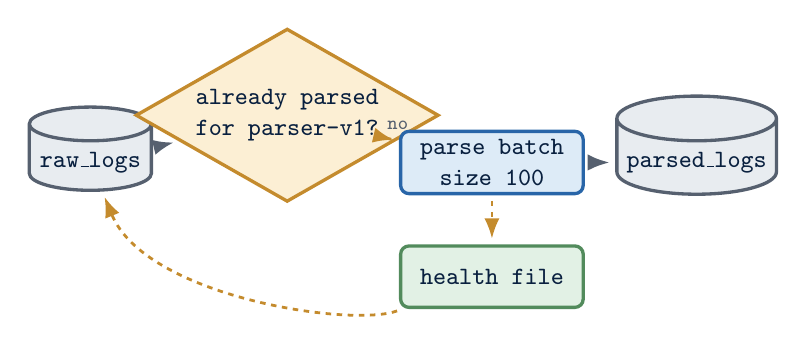
\begin{tikzpicture}[x=1cm,y=1cm]
  \node[db] (raw) at (1.5,2.7) {raw\_logs};
  \node[warn] (lookup) at (4.0,3.3) {already parsed\\for parser-v1?};
  \node[worker] (parse) at (6.6,2.7) {parse batch\\size 100};
  \node[db] (parsed) at (9.2,2.7) {parsed\_logs};
  \node[ok] (health) at (6.6,1.25) {health file};
  \draw[dbread] (raw)--(lookup);
  \draw[control] (lookup)--node[above,note]{no}(parse);
  \draw[dbwrite] (parse)--(parsed);
  \draw[control] (parse)--(health);
  \draw[control] (health) .. controls (4.8,.6) and (2.2,1.0) .. (raw);
\end{tikzpicture}
\end{frame}

\begin{frame}{Raw Text to Structured Event}
\centering
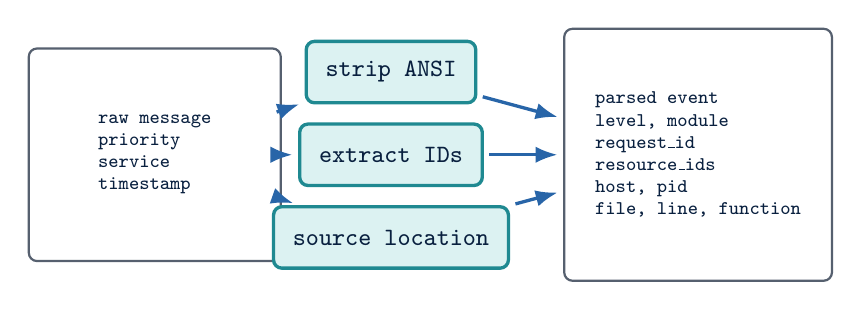
\begin{tikzpicture}[x=1cm,y=1cm]
  \node[artifact,minimum width=3.2cm,minimum height=2.7cm] (raw) at (2.1,2.45) {raw message\\priority\\service\\timestamp};
  \node[transform] (ansi) at (5.1,3.5) {strip ANSI};
  \node[transform] (ids) at (5.1,2.45) {extract IDs};
  \node[transform] (src) at (5.1,1.4) {source location};
  \node[artifact,minimum width=3.4cm,minimum height=3.2cm] (out) at (9.0,2.45) {parsed event\\level, module\\request\_id\\resource\_ids\\host, pid\\file, line, function};
  \draw[logflow] (raw)--(ansi);
  \draw[logflow] (raw)--(ids);
  \draw[logflow] (raw)--(src);
  \draw[logflow] (ansi)--(out);
  \draw[logflow] (ids)--(out);
  \draw[logflow] (src)--(out);
\end{tikzpicture}
\end{frame}

\begin{frame}{Extraction Graph}
\centering
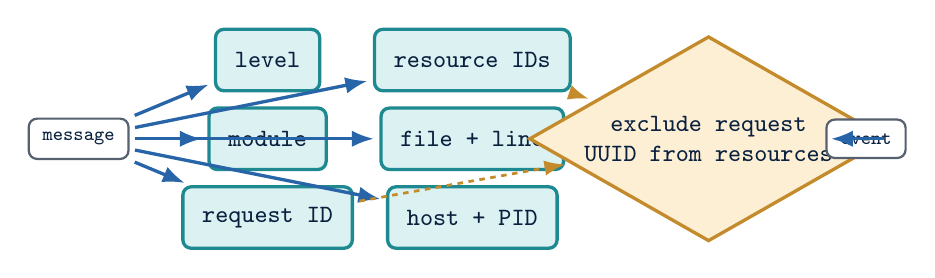
\begin{tikzpicture}[x=1cm,y=1cm]
  \node[artifact] (msg) at (1.2,2.55) {message};
  \node[transform] (level) at (3.6,3.55) {level};
  \node[transform] (module) at (3.6,2.55) {module};
  \node[transform] (req) at (3.6,1.55) {request ID};
  \node[transform] (res) at (6.2,3.55) {resource IDs};
  \node[transform] (loc) at (6.2,2.55) {file + line};
  \node[transform] (host) at (6.2,1.55) {host + PID};
  \node[warn] (exclude) at (9.2,2.55) {exclude request\\UUID from resources};
  \node[artifact] (event) at (11.2,2.55) {event};
  \foreach \n in {level,module,req,res,loc,host}{\draw[logflow] (msg)--(\n);}
  \draw[control] (req)--(exclude);
  \draw[control] (res)--(exclude);
  \draw[logflow] (exclude)--(event);
\end{tikzpicture}
\end{frame}

\begin{frame}{Parse Failure Preservation}
\centering
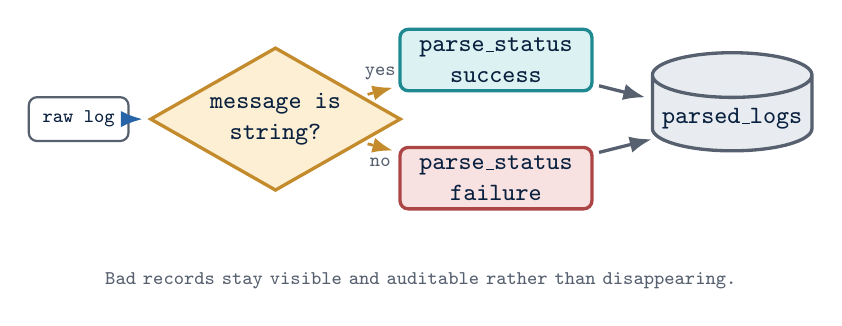
\begin{tikzpicture}[x=1cm,y=1cm]
  \node[artifact] (raw) at (1.7,2.6) {raw log};
  \node[warn] (valid) at (4.2,2.6) {message is\\string?};
  \node[transform] (ok) at (7.0,3.35) {parse\_status\\success};
  \node[err] (fail) at (7.0,1.85) {parse\_status\\failure};
  \node[db] (parsed) at (10.0,2.6) {parsed\_logs};
  \draw[logflow] (raw)--(valid);
  \draw[control] (valid)--node[above,note]{yes}(ok);
  \draw[control] (valid)--node[below,note]{no}(fail);
  \draw[dbwrite] (ok)--(parsed);
  \draw[dbwrite] (fail)--(parsed);
  \node[note,text width=8cm] at (6,.55) {Bad records stay visible and auditable rather than disappearing.};
\end{tikzpicture}
\end{frame}

\begin{frame}{Parser Idempotency and Versioning}
\centering
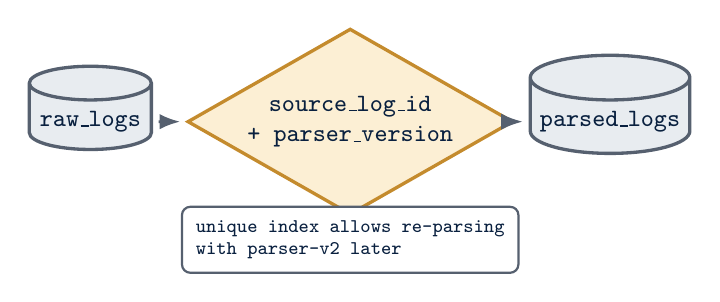
\begin{tikzpicture}[x=1cm,y=1cm]
  \node[db] (raw) at (2,2.5) {raw\_logs};
  \node[warn] (key) at (5.3,2.5) {source\_log\_id\\+ parser\_version};
  \node[db] (parsed) at (8.6,2.5) {parsed\_logs};
  \node[artifact] at (5.3,1.0) {unique index allows re-parsing\\with parser-v2 later};
  \draw[dbread] (raw)--(key);
  \draw[dbwrite] (key)--(parsed);
\end{tikzpicture}
\end{frame}

\section{9. Graph correlation: events to relationships}

\begin{frame}{Event Nodes and Correlation Edges}
\centering
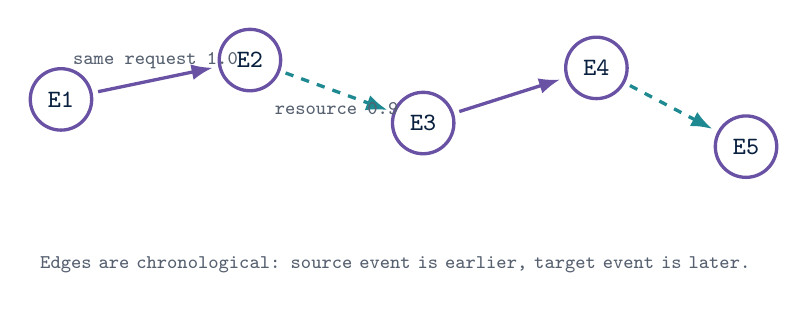
\begin{tikzpicture}[x=1cm,y=1cm]
  \node[event] (a) at (2,3.2) {E1};
  \node[event] (b) at (4.4,3.7) {E2};
  \node[event] (c) at (6.6,2.9) {E3};
  \node[event] (d) at (8.8,3.6) {E4};
  \node[event] (e) at (10.7,2.6) {E5};
  \draw[edgeReq] (a)--node[above,note]{same request 1.0}(b);
  \draw[edgeRes] (b)--node[below,note]{resource 0.9}(c);
  \draw[edgeReq] (c)--(d);
  \draw[edgeRes] (d)--(e);
  \node[note,text width=9cm] at (6.2,1.1) {Edges are chronological: source event is earlier, target event is later.};
\end{tikzpicture}
\end{frame}

\begin{frame}{Realistic Multi-Service Correlation Graph}
\centering
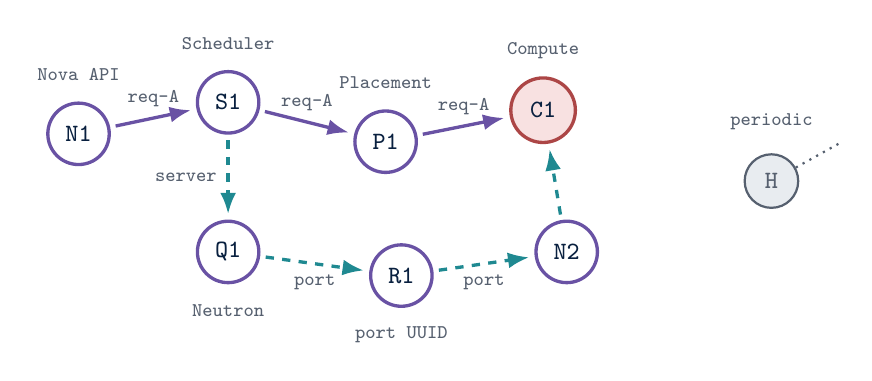
\begin{tikzpicture}[x=1cm,y=1cm]
  \node[event] (n1) at (1.3,3.4) {N1};
  \node[event] (n2) at (3.2,3.8) {S1};
  \node[event] (n3) at (5.2,3.3) {P1};
  \node[seed] (n4) at (7.2,3.7) {C1};
  \node[event] (n5) at (3.2,1.9) {Q1};
  \node[event] (n6) at (5.4,1.6) {R1};
  \node[event] (n7) at (7.5,1.9) {N2};
  \node[excluded] (n8) at (10.1,2.8) {H};
  \node[note] at (1.3,4.15) {Nova API};
  \node[note] at (3.2,4.55) {Scheduler};
  \node[note] at (5.2,4.05) {Placement};
  \node[note] at (7.2,4.45) {Compute};
  \node[note] at (3.2,1.15) {Neutron};
  \node[note] at (5.4,.85) {port UUID};
  \node[note] at (10.1,3.55) {periodic};
  \draw[edgeReq] (n1)--node[above,note]{req-A}(n2);
  \draw[edgeReq] (n2)--node[above,note]{req-A}(n3);
  \draw[edgeReq] (n3)--node[above,note]{req-A}(n4);
  \draw[edgeRes] (n2)--node[left,note]{server}(n5);
  \draw[edgeRes] (n5)--node[below,note]{port}(n6);
  \draw[edgeRes] (n6)--node[below,note]{port}(n7);
  \draw[edgeRes] (n7)--(n4);
  \draw[Slate,dotted,thick] (n8) -- ++(.9,.5);
\end{tikzpicture}
\end{frame}

\begin{frame}{Correlation Rule Windows}
\centering
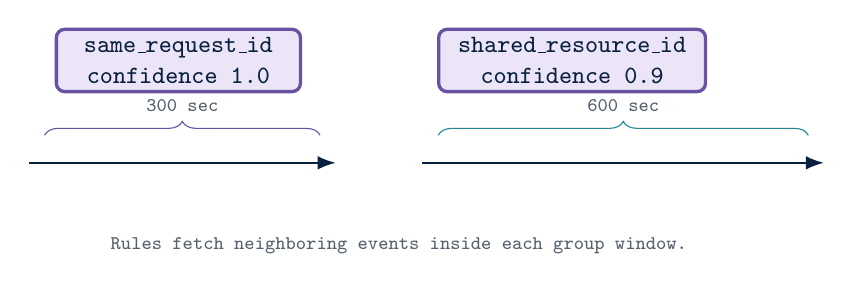
\begin{tikzpicture}[x=1cm,y=1cm]
  \node[graphlogic,minimum width=3.1cm] at (3.2,3.0) {same\_request\_id\\confidence 1.0};
  \node[graphlogic,minimum width=3.1cm] at (8.2,3.0) {shared\_resource\_id\\confidence 0.9};
  \draw[DeepNavy,thick,-{Latex}] (1.3,1.7) -- (5.2,1.7);
  \draw[DeepNavy,thick,-{Latex}] (6.3,1.7) -- (11.4,1.7);
  \draw[decorate,decoration={brace,amplitude=5pt},draw=Purple] (1.5,2.05)--node[above=5pt,note]{300 sec}(5.0,2.05);
  \draw[decorate,decoration={brace,amplitude=5pt},draw=Teal] (6.5,2.05)--node[above=5pt,note]{600 sec}(11.2,2.05);
  \node[note] at (6,.65) {Rules fetch neighboring events inside each group window.};
\end{tikzpicture}
\end{frame}

\begin{frame}{Transactional vs Periodic Groups}
\centering
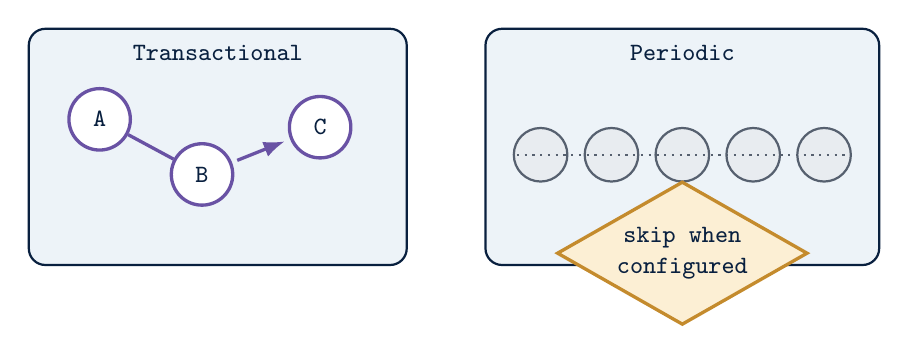
\begin{tikzpicture}[x=1cm,y=1cm]
  \node[zone,minimum width=4.8cm,minimum height=3cm] at (3.2,2.55) {};
  \node[smalltitle] at (3.2,3.75) {Transactional};
  \foreach \x/\y/\n in {1.7/2.9/A,3.0/2.2/B,4.5/2.8/C}{\node[event] (\n) at (\x,\y) {\n};}
  \draw[edgeReq] (A)--(B)--(C);
  \node[zone,minimum width=5.0cm,minimum height=3cm] at (9.1,2.55) {};
  \node[smalltitle] at (9.1,3.75) {Periodic};
  \foreach \x/\n in {7.3/H1,8.2/H2,9.1/H3,10.0/H4,10.9/H5}{\node[excluded] (\n) at (\x,2.45) {};}
  \draw[Slate,thick,dotted] (7.0,2.45)--(11.3,2.45);
  \node[warn] at (9.1,1.2) {skip when\\configured};
\end{tikzpicture}
\end{frame}

\section{10. Graph safety controls}

\begin{frame}{Before: Complete Pairwise Graph}
\centering
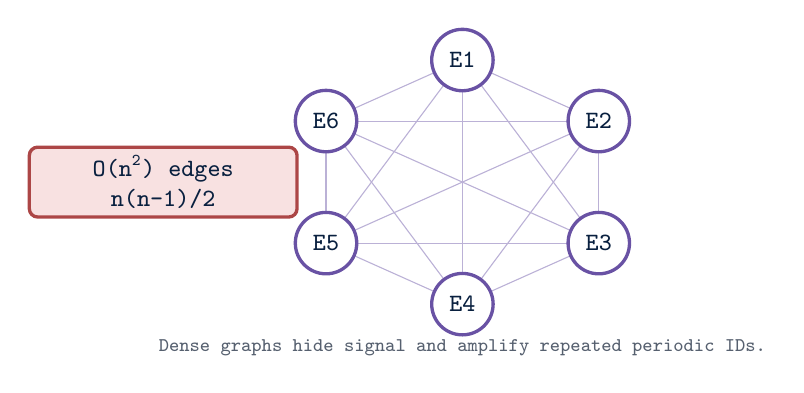
\begin{tikzpicture}[x=1cm,y=1cm]
  \coordinate (p1) at ({6+2.0*cos(90)},{2.55+1.55*sin(90)});
  \coordinate (p2) at ({6+2.0*cos(30)},{2.55+1.55*sin(30)});
  \coordinate (p3) at ({6+2.0*cos(-30)},{2.55+1.55*sin(-30)});
  \coordinate (p4) at ({6+2.0*cos(-90)},{2.55+1.55*sin(-90)});
  \coordinate (p5) at ({6+2.0*cos(-150)},{2.55+1.55*sin(-150)});
  \coordinate (p6) at ({6+2.0*cos(150)},{2.55+1.55*sin(150)});
  \begin{scope}[on background layer]
    \foreach \i in {1,...,5}{
      \pgfmathtruncatemacro{\s}{\i+1}
      \foreach \j in {\s,...,6}{\draw[Purple!45,thin,-{Latex[length=1.4mm]},shorten >=7pt,shorten <=7pt] (p\i)--(p\j);}
    }
  \end{scope}
  \foreach \i in {1,...,6}{\node[event] (e\i) at (p\i) {E\i};}
  \node[err,minimum width=3.4cm] at (2.2,2.55) {O(n\textsuperscript{2}) edges\\n(n-1)/2};
  \node[note] at (6,.45) {Dense graphs hide signal and amplify repeated periodic IDs.};
\end{tikzpicture}
\end{frame}

\begin{frame}{After: Consecutive-Only Chain}
\centering
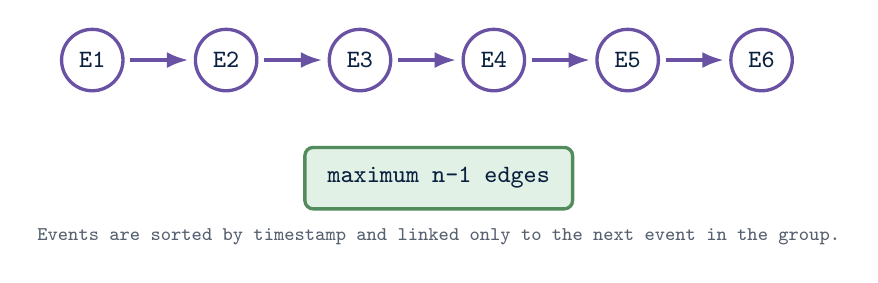
\begin{tikzpicture}[x=1cm,y=1cm]
  \foreach \i/\x in {1/1.6,2/3.3,3/5.0,4/6.7,5/8.4,6/10.1}{\node[event] (e\i) at (\x,2.6) {E\i};}
  \foreach \i/\j in {1/2,2/3,3/4,4/5,5/6}{\draw[edgeReq] (e\i)--(e\j);}
  \node[ok,minimum width=3.4cm] at (6,1.1) {maximum n-1 edges};
  \node[note] at (6,.35) {Events are sorted by timestamp and linked only to the next event in the group.};
\end{tikzpicture}
\end{frame}

\begin{frame}{Explosion Fix Decision Flow}
\centering
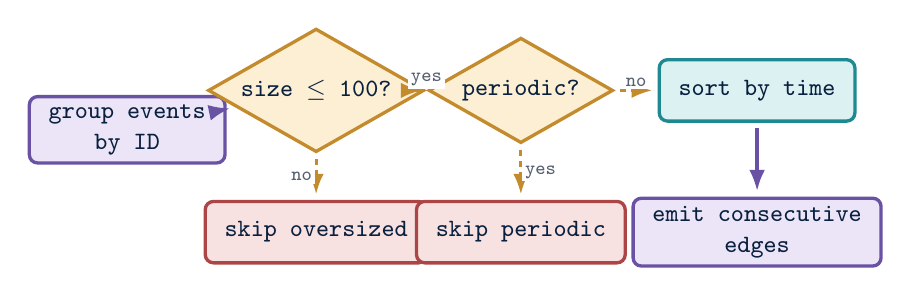
\begin{tikzpicture}[x=1cm,y=1cm]
  \node[graphlogic,minimum width=2.05cm] (group) at (1.25,2.75) {group events\\by ID};
  \node[warn,minimum width=2.0cm] (size) at (3.65,3.25) {size $\le$ 100?};
  \node[warn,minimum width=1.85cm] (periodic) at (6.25,3.25) {periodic?};
  \node[transform,minimum width=2.35cm] (sort) at (9.25,3.25) {sort by time};
  \node[graphlogic,minimum width=2.95cm] (edge) at (9.25,1.45) {emit consecutive\\edges};
  \node[err,minimum width=2.35cm] (skip1) at (3.65,1.45) {skip oversized};
  \node[err,minimum width=2.35cm] (skip2) at (6.25,1.45) {skip periodic};
  \draw[edgeReq] (group)--(size);
  \draw[control] (size)--node[above,note,fill=white,inner sep=1pt]{yes}(periodic);
  \draw[control] (size)--node[left,note,fill=white,inner sep=1pt]{no}(skip1);
  \draw[control] (periodic)--node[above,note,fill=white,inner sep=1pt]{no}(sort);
  \draw[control] (periodic)--node[right,note,fill=white,inner sep=1pt]{yes}(skip2);
  \draw[edgeReq] (sort)--(edge);
\end{tikzpicture}
\end{frame}

\begin{frame}{Observed Impact}
\centering
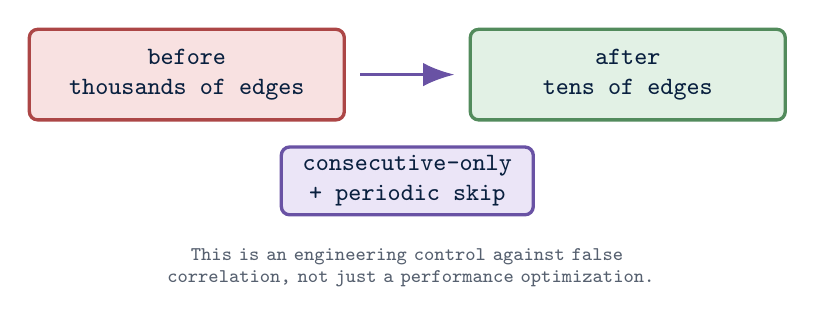
\begin{tikzpicture}[x=1cm,y=1cm]
  \node[err,minimum width=4cm,minimum height=1.15cm] at (3.2,3.0) {before\\thousands of edges};
  \node[ok,minimum width=4cm,minimum height=1.15cm] at (8.8,3.0) {after\\tens of edges};
  \draw[Purple,very thick,-{Latex[length=4mm]}] (5.4,3.0)--(6.6,3.0);
  \node[graphlogic,minimum width=3.2cm] at (6,1.65) {consecutive-only\\+ periodic skip};
  \node[note,text width=9cm] at (6,.55) {This is an engineering control against false correlation, not just a performance optimization.};
\end{tikzpicture}
\end{frame}

\section{11. Incident detection: suspicious seed events}

\begin{frame}{Incident Seed Rule Engine}
\centering
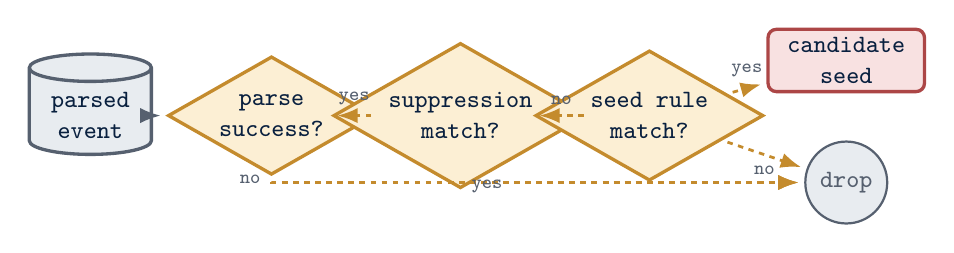
\begin{tikzpicture}[x=1cm,y=1cm]
  \node[db] (p) at (1.2,2.65) {parsed\\event};
  \node[warn] (success) at (3.5,2.65) {parse\\success?};
  \node[warn] (suppress) at (5.9,2.65) {suppression\\match?};
  \node[warn] (rules) at (8.3,2.65) {seed rule\\match?};
  \node[err] (seed) at (10.8,3.35) {candidate\\seed};
  \node[excluded] (drop) at (10.8,1.8) {drop};
  \draw[dbread] (p)--(success);
  \draw[control] (success)--node[above,note]{yes}(suppress);
  \draw[control] (success)|-node[pos=.25,left,note]{no}(drop);
  \draw[control] (suppress)--node[above,note]{no}(rules);
  \draw[control] (suppress)|-node[pos=.25,right,note]{yes}(drop);
  \draw[control] (rules)--node[above,note]{yes}(seed);
  \draw[control] (rules)--node[below,note]{no}(drop);
\end{tikzpicture}
\end{frame}

\begin{frame}{Accepted Seed Decision Tree}
\centering
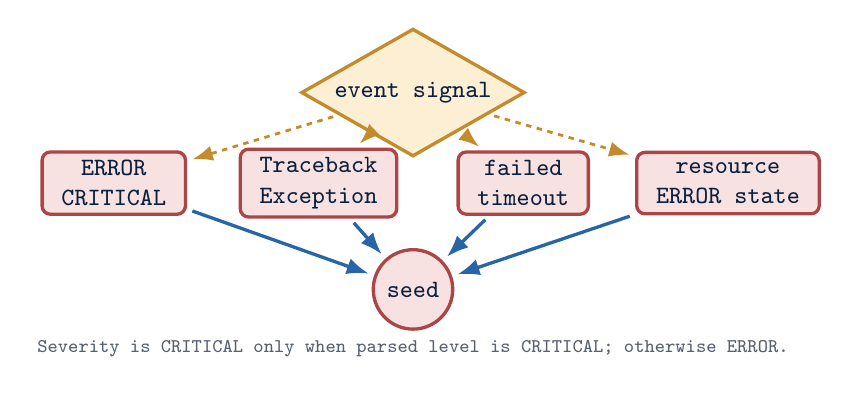
\begin{tikzpicture}[x=1cm,y=1cm]
  \node[warn] (root) at (6,3.6) {event signal};
  \node[err] (lvl) at (2.2,2.45) {ERROR\\CRITICAL};
  \node[err] (trace) at (4.8,2.45) {Traceback\\Exception};
  \node[err] (fail) at (7.4,2.45) {failed\\timeout};
  \node[err] (res) at (10.0,2.45) {resource\\ERROR state};
  \node[seed] (seed) at (6,1.1) {seed};
  \foreach \n in {lvl,trace,fail,res}{\draw[control] (root)--(\n); \draw[logflow] (\n)--(seed);}
  \node[note] at (6,.35) {Severity is CRITICAL only when parsed level is CRITICAL; otherwise ERROR.};
\end{tikzpicture}
\end{frame}

\begin{frame}{Rejected False Positives}
\centering
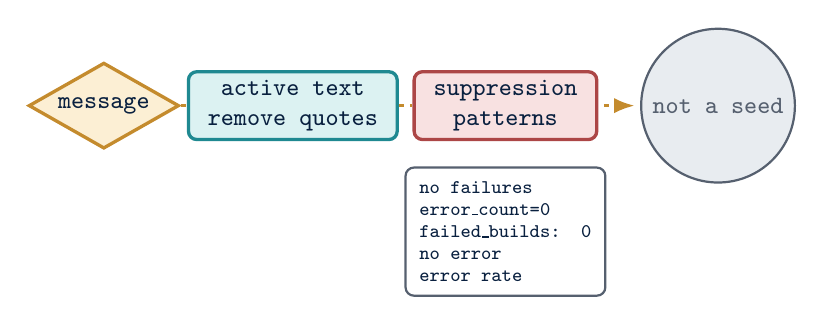
\begin{tikzpicture}[x=1cm,y=1cm]
  \node[warn] (msg) at (1.6,2.65) {message};
  \node[transform] (active) at (4.0,2.65) {active text\\remove quotes};
  \node[err] (patterns) at (6.7,2.65) {suppression\\patterns};
  \node[excluded] (drop) at (9.4,2.65) {not a seed};
  \node[artifact] at (6.7,1.05) {no failures\\error\_count=0\\failed\_builds: 0\\no error\\error rate};
  \draw[control] (msg)--(active)--(patterns)--(drop);
\end{tikzpicture}
\end{frame}

\section{12. Incident construction: bounded subgraphs}

\begin{frame}{Bounded Traversal Around Seed}
\centering
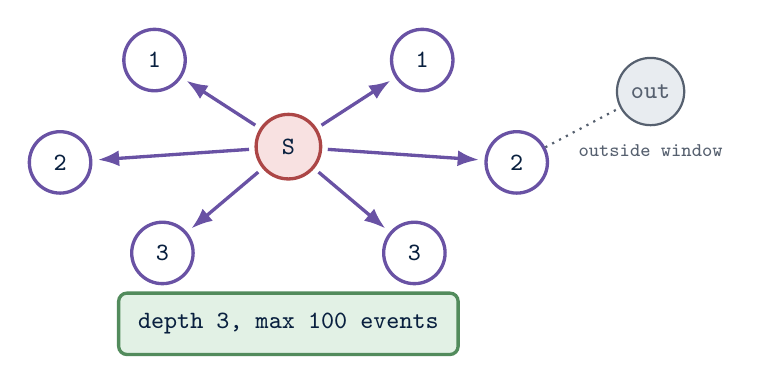
\begin{tikzpicture}[x=1cm,y=1cm]
  \node[seed] (s) at (6,2.6) {S};
  \node[event] (a) at (4.3,3.7) {1};
  \node[event] (b) at (7.7,3.7) {1};
  \node[event] (c) at (3.1,2.4) {2};
  \node[event] (d) at (8.9,2.4) {2};
  \node[event] (e) at (4.4,1.25) {3};
  \node[event] (f) at (7.6,1.25) {3};
  \node[excluded] (x) at (10.6,3.3) {out};
  \foreach \n in {a,b,c,d,e,f}{\draw[edgeReq] (s)--(\n);}
  \draw[Slate,dotted,thick] (d)--(x);
  \node[note] at (10.6,2.55) {outside window};
  \node[ok,minimum width=3.0cm] at (6,.35) {depth 3, max 100 events};
\end{tikzpicture}
\end{frame}

\begin{frame}{Incident Window}
\centering
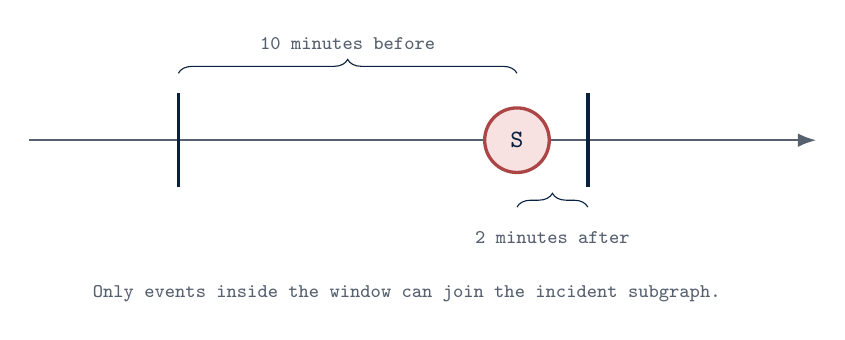
\begin{tikzpicture}[x=1cm,y=1cm]
  \draw[Slate,thick,-{Latex}] (1.2,2.5)--(11.2,2.5);
  \node[seed] at (7.4,2.5) {S};
  \draw[DeepNavy,very thick] (3.1,1.9)--(3.1,3.1);
  \draw[DeepNavy,very thick] (8.3,1.9)--(8.3,3.1);
  \draw[decorate,decoration={brace,amplitude=5pt},draw=DeepNavy] (3.1,3.35)--node[above=5pt,note]{10 minutes before}(7.4,3.35);
  \draw[decorate,decoration={brace,amplitude=5pt},draw=DeepNavy] (7.4,1.65)--node[below=5pt,note]{2 minutes after}(8.3,1.65);
  \node[note] at (6,.55) {Only events inside the window can join the incident subgraph.};
\end{tikzpicture}
\end{frame}

\begin{frame}{Correlation Is Not Causality}
\centering
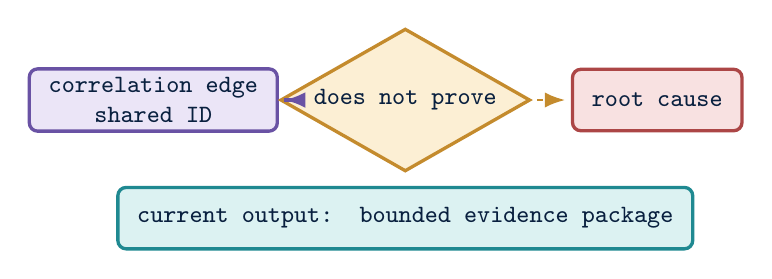
\begin{tikzpicture}[x=1cm,y=1cm]
  \node[graphlogic] (corr) at (2.8,2.6) {correlation edge\\shared ID};
  \node[warn] (not) at (6,2.6) {does not prove};
  \node[err] (cause) at (9.2,2.6) {root cause};
  \draw[edgeReq] (corr)--(not);
  \draw[control] (not)--(cause);
  \node[transform,minimum width=3.8cm] at (6,1.1) {current output: bounded evidence package};
\end{tikzpicture}
\end{frame}

\section{13. Worker reliability}

\begin{frame}{Before: Repeated First-Page Scanning}
\centering
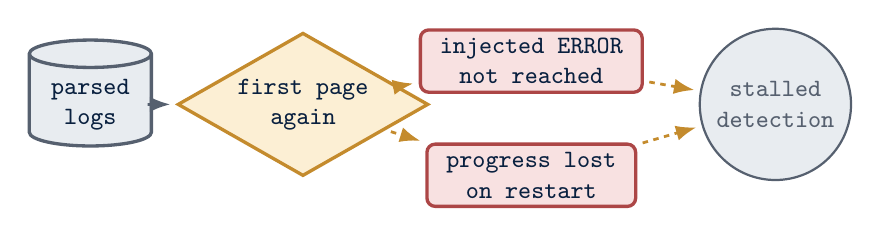
\begin{tikzpicture}[x=1cm,y=1cm]
  \node[db] (parsed) at (1.4,2.7) {parsed\\logs};
  \node[warn] (page) at (4.1,2.7) {first page\\again};
  \node[err] (miss) at (7.0,3.25) {injected ERROR\\not reached};
  \node[err] (mem) at (7.0,1.8) {progress lost\\on restart};
  \node[excluded] (idle) at (10.1,2.7) {stalled\\detection};
  \draw[dbread] (parsed)--(page);
  \draw[control] (page)--(miss);
  \draw[control] (page)--(mem);
  \draw[control] (miss)--(idle);
  \draw[control] (mem)--(idle);
\end{tikzpicture}
\end{frame}

\begin{frame}{After: Persistent worker\_state}
\centering
\begin{tikzpicture}[x=1cm,y=1cm]
  \node[db] (parsed) at (1.2,2.8) {parsed\\logs};
  \node[worker] (worker) at (3.8,2.8) {incident\\worker};
  \node[warn] (order) at (6.3,3.35) {sort by\\parsed\_at + \_id};
  \node[ok] (save) at (8.8,3.35) {save after\\batch};
  \node[db] (state) at (11.1,3.35) {worker\\state};
  \node[ok] (resume) at (6.3,1.5) {resume\\after checkpoint};
  \draw[dbread] (parsed)--(worker);
  \draw[control] (worker)--(order);
  \draw[control] (order)--(save);
  \draw[dbwrite] (save)--(state);
  \draw[dbread] (state) |- (resume);
  \draw[control] (resume)--(worker);
\end{tikzpicture}
\end{frame}

\section{14. Enrichment: deterministic evidence package}

\begin{frame}{Enrichment Worker Architecture}
\centering
\begin{tikzpicture}[x=1cm,y=1cm]
  \node[db] (inc) at (1.4,2.7) {incidents\\candidate};
  \node[worker] (w) at (3.8,2.7) {enrichment\\worker};
  \node[db] (parsed) at (6.3,3.45) {parsed\\events};
  \node[db] (edges) at (6.3,1.95) {event\\edges};
  \node[transform] (derive) at (8.8,2.7) {derive\\timeline\\counts\\summaries};
  \node[db] (out) at (11.2,2.7) {incidents\\enriched};
  \draw[dbread] (inc)--(w);
  \draw[dbread] (w)--(parsed);
  \draw[dbread] (w)--(edges);
  \draw[logflow] (w)--(derive);
  \draw[dbwrite] (derive)--(out);
\end{tikzpicture}
\end{frame}

\begin{frame}{Enriched Incident Timeline}
\centering
\begin{tikzpicture}[x=1cm,y=1cm]
  \draw[Slate,thick,-{Latex}] (1.0,2.5)--(11.8,2.5);
  \foreach \x/\id/\svc/\lvl in {1.7/E1/API/INFO,3.5/E2/Scheduler/WARN,5.3/E3/Placement/INFO,7.1/S/Compute/ERROR,8.9/E5/Neutron/WARN,10.7/E6/Compute/ERROR}{
    \node[event] (\id) at (\x,2.5) {\id};
    \node[note] at (\x,1.75) {\svc};
    \node[note] at (\x,3.22) {\lvl};
  }
  \node[seed] at (7.1,2.5) {S};
  \draw[edgeReq] (E1) to[bend left=28] node[above,note]{req-A} (S);
  \draw[edgeRes] (E2) to[bend right=26] node[below,note]{server UUID} (E5);
\end{tikzpicture}
\end{frame}

\begin{frame}{Enriched Incident Document}
\centering
\begin{tikzpicture}[x=1cm,y=1cm]
  \node[db] (inc) at (1.4,2.5) {incident};
  \foreach \txt/\x/\y in {
    timeline/4.0/3.55,services/6.4/3.55,request IDs/8.8/3.55,
    resource IDs/4.0/2.45,error count/6.4/2.45,warning count/8.8/2.45,
    summary/4.0/1.35,impact summary/6.4/1.35,evidence summary/8.8/1.35}
    {\node[transform,minimum width=2.0cm] at (\x,\y) {\txt};}
  \node[ok] at (11.2,2.45) {status\\enriched};
\end{tikzpicture}
\end{frame}

\section{15. MongoDB collection architecture}

\begin{frame}{Collection Relationship Map}
\centering
\begin{tikzpicture}[x=1cm,y=1cm]
  \node[db] (raw) at (1.2,3.2) {raw\_logs};
  \node[db] (parsed) at (3.8,3.2) {parsed\_logs};
  \node[db] (edges) at (6.4,3.2) {event\_edges};
  \node[db] (inc) at (9.0,3.2) {incidents};
  \node[db] (state) at (11.4,1.8) {worker\\state};
  \draw[dbwrite] (raw)--node[above,note]{source\_log\_id}(parsed);
  \draw[dbwrite] (parsed)--node[above,note]{source/target IDs}(edges);
  \draw[dbread] (parsed) to[bend right=18] node[below,note]{event\_ids}(inc);
  \draw[dbread] (edges) to[bend left=18] node[above,note]{edge\_ids}(inc);
  \draw[control] (inc)--(state);
  \draw[control] (state)--(inc);
\end{tikzpicture}
\end{frame}

\begin{frame}{Indexes and Version Fields}
\centering
\begin{tikzpicture}[x=1cm,y=1cm]
  \node[artifact] at (2.2,3.4) {raw\_logs\\uniq boot\_id + cursor};
  \node[artifact] at (5.0,3.4) {parsed\_logs\\uniq source + parser};
  \node[artifact] at (8.0,3.4) {event\_edges\\uniq edge + reason + version};
  \node[artifact] at (10.8,3.4) {incidents\\uniq seed + incident version};
  \node[artifact] at (3.6,1.7) {parser-v1};
  \node[artifact] at (6.0,1.7) {correlation-v1};
  \node[artifact] at (8.4,1.7) {incident-v1};
  \node[artifact] at (10.8,1.7) {enrichment-v1};
\end{tikzpicture}
\end{frame}

\begin{frame}{Immutable vs Mutable Collections}
\centering
\begin{tikzpicture}[x=1cm,y=1cm]
  \node[ok,minimum width=4.2cm] at (3.3,3.1) {append / set-on-insert};
  \node[db] at (2.1,1.95) {raw};
  \node[db] at (3.5,1.95) {parsed};
  \node[db] at (4.9,1.95) {edges};
  \node[warn,minimum width=4.2cm] at (8.8,3.1) {updated by workflow};
  \node[db] at (8.0,1.95) {incidents};
  \node[db] at (9.6,1.95) {state};
  \node[note] at (6,.65) {Raw evidence is preserved; incident documents mature from candidate to enriched.};
\end{tikzpicture}
\end{frame}

\section{16. Failure containment}

\begin{frame}{Reliability Shield}
\centering
\begin{tikzpicture}[x=1cm,y=1cm]
  \node[zone,minimum width=7.8cm,minimum height=4.3cm] at (6,2.45) {};
  \node[transform,minimum width=2.4cm] at (6,2.45) {evidence\\pipeline};
  \node[ok] at (3,3.6) {dedupe};
  \node[ok] at (6,3.8) {healthchecks};
  \node[ok] at (9,3.6) {restart policy};
  \node[ok] at (3,1.35) {versions};
  \node[ok] at (6,1.1) {checkpoints};
  \node[ok] at (9,1.35) {persistent volume};
  \draw[control] (3,3.6)--(6,2.45);
  \draw[control] (6,3.8)--(6,2.45);
  \draw[control] (9,3.6)--(6,2.45);
  \draw[control] (3,1.35)--(6,2.45);
  \draw[control] (6,1.1)--(6,2.45);
  \draw[control] (9,1.35)--(6,2.45);
\end{tikzpicture}
\end{frame}

\begin{frame}{Failure Containment}
\centering
\begin{tikzpicture}[x=1cm,y=1cm]
  \node[err] (backend) at (2.2,3.2) {backend down};
  \node[err] (parse) at (2.2,1.8) {parse error};
  \node[err] (worker) at (6.0,3.2) {worker restart};
  \node[err] (dup) at (6.0,1.8) {duplicate record};
  \node[ok] (contain) at (9.6,2.5) {contained\\no data loss};
  \draw[control] (backend)--node[above,note]{retry + no cursor advance}(contain);
  \draw[control] (parse)--node[below,note]{failure preserved}(contain);
  \draw[control] (worker)--node[above,note]{checkpoint/version}(contain);
  \draw[control] (dup)--node[below,note]{unique indexes}(contain);
\end{tikzpicture}
\end{frame}

\section{17. Current versus future boundary}

\begin{frame}{Current and Future Capability Boundary}
\centering
\begin{tikzpicture}[x=1cm,y=1cm]
  \node[zone,minimum width=5.5cm,minimum height=3.8cm] at (3.1,2.45) {};
  \node[smalltitle] at (3.1,3.95) {Current};
  \foreach \txt/\x/\y in {ingestion/1.7/3.2,parsing/3.1/3.2,correlation/4.5/3.2,seeds/2.4/2.1,enrichment/3.8/2.1}{\node[ok,minimum width=1.4cm] at (\x,\y) {\txt};}
  \node[trust,minimum width=5.5cm,minimum height=3.8cm] at (9.1,2.45) {};
  \node[smalltitle,text=Slate] at (9.1,3.95) {Future};
  \foreach \txt/\x/\y in {vectors/7.5/3.2,embeddings/9.1/3.2,reranker/10.8/3.2,provider/8.2/2.1,Horizon/10.0/2.1}{\node[future,minimum width=1.4cm] at (\x,\y) {\txt};}
\end{tikzpicture}
\end{frame}

\section{18. Future AI/RAG layer}

\begin{frame}{Selective Vectorization Funnel}
\centering
\begin{tikzpicture}[x=1cm,y=1cm]
  \node[db] (mongoF) at (1.2,3.1) {Mongo};
  \node[artifact,minimum width=2.3cm] (rawF) at (3.5,3.65) {all raw logs};
  \node[warn,minimum width=2.5cm] (filterF) at (5.95,3.0) {filter high\\signal};
  \node[future,minimum width=2.5cm] (embedF) at (8.35,3.58) {embedding\\request};
  \node[future,minimum width=2.5cm] (chromaF) at (10.8,3.0) {Chroma\\vectors};
  \node[artifact] at (5.8,1.4) {ERROR\\WARNING\\traceback\\enriched incident\\summary\\correlated chunk};
  \draw[dbread] (mongoF.east) -- (rawF.west);
  \draw[control] (rawF.east) -- (filterF.north west);
  \draw[futureline] (filterF.north east) -- (embedF.west);
  \draw[futureline] (embedF.east) -- (chromaF.west);
\end{tikzpicture}
\end{frame}

\begin{frame}{Retrieval Architecture}
\centering
\begin{tikzpicture}[x=1cm,y=1cm]
  \node[transform] (inc) at (1.6,2.8) {selected\\incident};
  \node[db] (mongo) at (4.0,3.45) {Mongo\\truth};
  \node[future] (chroma) at (4.0,2.0) {Chroma\\similarity};
  \node[future] (rerank) at (6.8,2.7) {reranker};
  \node[future] (ctx) at (9.5,2.7) {grounded\\context};
  \draw[dbread] (inc)--(mongo);
  \draw[futureline] (inc)--(chroma);
  \draw[futureline] (mongo)--(rerank);
  \draw[futureline] (chroma)--(rerank);
  \draw[futureline] (rerank)--(ctx);
  \node[note] at (6,.65) {Retrieved vectors point back to MongoDB evidence IDs.};
\end{tikzpicture}
\end{frame}

\section{19. Future local provider node}

\begin{frame}{Future Local Provider Node}
\centering
\begin{tikzpicture}[x=1cm,y=1cm]
  \node[machine,minimum width=8.6cm,minimum height=4.4cm] at (6,2.45) {};
  \node[smalltitle,text=Slate] at (6,4.25) {Optional local AI node (future)};
  \node[future] (api) at (2.9,3.25) {auth API};
  \node[future] (emb) at (5.2,3.25) {sentence\\transformer};
  \node[future] (cuda) at (7.6,3.25) {CUDA\\RTX 4070};
  \node[future] (rerank) at (4.0,1.75) {reranker};
  \node[future] (ollama) at (6.6,1.75) {local/provider\\LLM};
  \node[future] (health) at (9.0,1.75) {health\\checks};
  \draw[futureline] (api)--(emb)--(cuda);
  \draw[futureline] (api)--(rerank)--(ollama);
  \draw[futureline] (api)--(health);
  \node[note] at (6,.55) {MongoDB remains source of truth; optional providers compute embeddings, ranking, or generation.};
\end{tikzpicture}
\end{frame}

\section{20. Future grounded AI workflow}

\begin{frame}{Grounded RCA Generation Flow}
\centering
\begin{tikzpicture}[x=1cm,y=1cm]
  \node[svc] (user) at (1.2,2.8) {user selects\\incident};
  \node[graphlogic] (graph) at (3.5,3.4) {load incident\\graph};
  \node[future] (query) at (5.9,3.4) {vector query};
  \node[future] (chroma) at (8.2,3.4) {similar\\evidence};
  \node[future] (rerank) at (5.9,1.8) {rerank};
  \node[future] (llm) at (8.2,1.8) {LLM evidence\\package};
  \node[future] (ans) at (10.7,2.6) {answer with\\event refs};
  \draw[logflow] (user)--(graph);
  \draw[futureline] (graph)--(query)--(chroma)--(rerank)--(llm)--(ans);
  \draw[futureline] (graph)--(llm);
\end{tikzpicture}
\end{frame}

\begin{frame}{Unsupported Claim Gate}
\centering
\begin{tikzpicture}[x=1cm,y=1cm]
  \node[future] (claim) at (2,2.7) {LLM claim};
  \node[warn] (ref) at (5,2.7) {linked to\\event evidence?};
  \node[ok] (keep) at (8.4,3.35) {allow with\\reference};
  \node[err] (block) at (8.4,1.85) {reject or\\ask for evidence};
  \draw[futureline] (claim)--(ref);
  \draw[control] (ref)--node[above,note]{yes}(keep);
  \draw[control] (ref)--node[below,note]{no}(block);
\end{tikzpicture}
\end{frame}

\section{21. Horizon dashboard and operator workflow}

\begin{frame}{Future Horizon RCA Copilot Tab}
\centering
\begin{tikzpicture}[x=1cm,y=1cm]
  \node[future,minimum width=10.8cm,minimum height=4.35cm] at (6,2.45) {};
  \node[smalltitle,text=Slate] at (6,4.25) {Horizon RCA Copilot tab};
  \node[future,minimum width=2.3cm] at (2.3,3.25) {incident list};
  \node[future,minimum width=2.8cm] at (5.2,3.25) {interactive graph};
  \node[future,minimum width=2.3cm] at (8.4,3.25) {timeline};
  \node[future,minimum width=2.3cm] at (10.8,3.25) {settings};
  \node[future,minimum width=2.8cm] at (4.1,1.75) {evidence panel};
  \node[future,minimum width=3.0cm] at (7.4,1.75) {AI explanation};
  \node[future,minimum width=2.3cm] at (10.5,1.75) {endpoint test};
\end{tikzpicture}
\end{frame}

\begin{frame}{Browser-to-Backend Flow}
\centering
\begin{tikzpicture}[x=1cm,y=1cm]
  \node[future] (browser) at (1.5,2.8) {Horizon\\browser};
  \node[svc] (api) at (4.3,2.8) {RCA backend};
  \node[db] (mongo) at (7.1,3.45) {Mongo};
  \node[future] (msi) at (7.1,2.0) {provider\\adapter};
  \node[future] (ollama) at (10,2.0) {AI backend};
  \draw[futureline] (browser)--node[above,note]{HTTPS/API}(api);
  \draw[dbread] (api)--(mongo);
  \draw[futureline] (api)--node[below,note]{Tailscale}(msi);
  \draw[futureline] (msi)--(ollama);
  \draw[err,draw=MutedRed,thick,dashed] (browser) to[bend right=20] node[below,note]{no direct call} (ollama);
\end{tikzpicture}
\end{frame}

\section{22. Operator investigation journey}

\begin{frame}{Operator Storyboard}
\centering
\begin{tikzpicture}[x=1cm,y=1cm]
  \tikzset{
    storybase/.style={rounded corners=6pt,very thick,align=center,text=DeepNavy,
      font=\small,minimum width=2.42cm,minimum height=1.36cm,inner sep=6pt},
    storynum/.style={circle,fill=white,draw=DeepNavy,line width=.8pt,
      font=\bfseries\small,text=DeepNavy,minimum size=.38cm,inner sep=0pt},
    storyicon/.style={font=\bfseries\large,text=DeepNavy,align=center},
    storyarrow/.style={-{Latex[length=3.4mm,width=2.5mm]},line width=1.35pt,draw=DeepNavy},
    storyfuture/.style={dash pattern=on 5pt off 3pt}
  }

  \node[storybase,draw=MutedRed,fill=SoftRed] (s1) at (1.55,4.35) {
    \strut\\[-4pt]Incident\\detected};
  \node[storynum] at ($(s1.north west)+(.25,-.25)$) {1};
  \node[storyicon] at ($(s1.north)+(0,-.27)$) {!};

  \node[storybase,draw=MediumBlue,fill=SoftBlue] (s2) at (4.58,4.35) {\strut\\[-4pt]Open RCA\\Copilot};
  \node[storynum] at ($(s2.north west)+(.25,-.25)$) {2};
  \node[storyicon] at ($(s2.north)+(0,-.27)$) {$\Box$};

  \node[storybase,draw=Purple,fill=SoftPurple] (s3) at (7.61,4.35) {\strut\\[-4pt]Inspect\\graph};
  \node[storynum] at ($(s3.north west)+(.25,-.25)$) {3};
  \node[storyicon] at ($(s3.north)+(0,-.27)$) {$\bullet\!-\!\bullet$};

  \node[storybase,draw=Purple,fill=SoftPurple] (s4) at (10.64,4.35) {\strut\\[-4pt]Select\\event};
  \node[storynum] at ($(s4.north west)+(.25,-.25)$) {4};
  \node[storyicon] at ($(s4.north)+(0,-.27)$) {$\triangleright$};

  \node[storybase,draw=MediumBlue,fill=SoftBlue] (s5) at (10.64,1.72) {\strut\\[-4pt]Review\\evidence};
  \node[storynum] at ($(s5.north west)+(.25,-.25)$) {5};
  \node[storyicon] at ($(s5.north)+(0,-.27)$) {$i$};

  \node[storybase,storyfuture,draw=Teal,fill=SoftTeal] (s6) at (7.61,1.72) {\strut\\[-4pt]Request AI\\explanation};
  \node[storynum] at ($(s6.north west)+(.25,-.25)$) {6};
  \node[storyicon] at ($(s6.north)+(0,-.27)$) {AI};

  \node[storybase,storyfuture,draw=Teal,fill=SoftTeal] (s7) at (4.58,1.72) {\strut\\[-4pt]Review\\context};
  \node[storynum] at ($(s7.north west)+(.25,-.25)$) {7};
  \node[storyicon] at ($(s7.north)+(0,-.27)$) {RAG};

  \node[storybase,draw=MutedGreen,fill=SoftGreen] (s8) at (1.55,1.72) {\strut\\[-4pt]Validate\\conclusion};
  \node[storynum] at ($(s8.north west)+(.25,-.25)$) {8};
  \node[storyicon] at ($(s8.north)+(0,-.27)$) {OK};

  \draw[storyarrow] (s1.east) -- (s2.west);
  \draw[storyarrow] (s2.east) -- (s3.west);
  \draw[storyarrow] (s3.east) -- (s4.west);
  \draw[storyarrow,rounded corners=7pt] (s4.south) -- ++(0,-.55) -- (s5.north);
  \draw[storyarrow] (s5.west) -- (s6.east);
  \draw[storyarrow,storyfuture] (s6.west) -- (s7.east);
  \draw[storyarrow,storyfuture] (s7.west) -- (s8.east);

  \node[draw=DeepNavy,rounded corners=4pt,fill=white,inner sep=5pt,anchor=north east] at (12.25,6.70) {
    \begin{tabular}{@{}ll@{}}
      \tikz{\draw[DeepNavy,line width=1.1pt] (0,0)--(.48,0);} & \small implemented\\
      \tikz{\draw[DeepNavy,line width=1.1pt,dash pattern=on 4pt off 2pt] (0,0)--(.48,0);} & \small future
    \end{tabular}
  };
\end{tikzpicture}
\end{frame}

\section{23. Final architecture}

\begin{frame}{Overall Architecture — Two-Machine RCA Copilot}
\centering
\begin{tikzpicture}[x=1cm,y=1cm]
  \tikzset{
    archzone/.style={draw=DeepNavy,line width=1.15pt,rounded corners=6pt,fill=LightBG,inner sep=5pt},
    layer/.style={draw=DeepNavy!38,line width=.75pt,rounded corners=4pt,fill=white,inner sep=4pt},
    layerfuture/.style={layer,dash pattern=on 5pt off 3pt},
    archlabel/.style={font=\bfseries\small,text=DeepNavy,fill=LightBG,inner sep=1.5pt},
    nodelabel/.style={font=\small,text=DeepNavy,align=center},
    shortlabel/.style={font=\small,text=DeepNavy,fill=white,inner sep=1.2pt},
    flowlabel/.style={font=\small,text=DeepNavy,fill=white,inner sep=1.1pt,anchor=east},
    item/.style={draw=MediumBlue,line width=1.05pt,rounded corners=4pt,fill=SoftBlue,
      font=\small,text=DeepNavy,align=center,minimum height=.58cm,inner xsep=4pt},
    storeitem/.style={draw=Slate,line width=1.05pt,rounded corners=4pt,fill=SoftSlate,
      font=\small,text=DeepNavy,align=center,minimum height=.50cm,inner xsep=3pt},
    futureitem/.style={draw=DeepNavy,line width=1.05pt,dash pattern=on 5pt off 3pt,
      rounded corners=4pt,fill=white,font=\small,text=DeepNavy,align=center,
      minimum height=.58cm,inner xsep=4pt},
    solidflow/.style={-{Latex[length=3mm,width=2.2mm]},line width=1.15pt,draw=MediumBlue},
    dataflow/.style={-{Latex[length=3mm,width=2.2mm]},line width=1.15pt,draw=Slate},
    detectflow/.style={-{Latex[length=3mm,width=2.2mm]},line width=1.2pt,draw=MutedRed},
    futureflow/.style={-{Latex[length=3mm,width=2.2mm]},line width=1.15pt,dash pattern=on 5pt off 3pt,draw=Teal},
    requestflow/.style={{Latex[length=2.6mm,width=2mm]}-{Latex[length=2.6mm,width=2mm]},line width=1.15pt,dash pattern=on 5pt off 3pt,draw=DeepNavy}
  }

  \node[archzone,minimum width=8.12cm,minimum height=6.12cm] (mac) at (4.22,3.12) {};
  \node[archlabel] at (4.22,6.22) {MacBook implemented system};
  \node[archzone,minimum width=1.12cm,minimum height=6.12cm,fill=white] (tail) at (8.93,3.12) {};
  \node[font=\bfseries\small,text=DeepNavy,align=center,rotate=90] at (8.93,3.12) {Private API Boundary};
  \node[font=\bfseries\small,text=DeepNavy,align=center,fill=white,inner sep=1pt] at (8.93,6.18) {Tailscale};
  \node[archzone,dash pattern=on 5pt off 3pt,minimum width=3.38cm,minimum height=6.12cm] (msi) at (11.55,3.12) {};
  \node[archlabel] at (11.55,6.22) {future AI provider system};

  \node[layer,minimum width=7.55cm,minimum height=.92cm] at (4.22,5.47) {};
  \node[shortlabel,anchor=west] at (.72,5.86) {OpenStack};
  \foreach \name/\x in {Nova/2.05,Neutron/3.45,Keystone/4.95,Placement/6.60}
    \node[item,minimum width=1.18cm] at (\x,5.47) {\name};

  \node[layer,minimum width=7.55cm,minimum height=.92cm] at (4.22,4.37) {};
  \node[shortlabel,anchor=west] at (.72,4.76) {Ingestion};
  \node[item,draw=Slate,fill=SoftSlate,minimum width=1.22cm] (journal) at (1.93,4.37) {journald};
  \node[item,minimum width=1.55cm] (collector) at (3.68,4.37) {host\\collector};
  \node[item,minimum width=1.65cm] (api) at (5.78,4.37) {FastAPI\\backend};

  \node[layer,minimum width=7.55cm,minimum height=2.22cm] at (4.22,2.92) {};
  \node[shortlabel,anchor=west] at (.72,3.88) {Evidence};
  \node[storeitem,minimum width=1.62cm] (raw) at (2.05,3.45) {raw logs};
  \node[storeitem,minimum width=1.62cm] (parsed) at (2.05,2.95) {parsed events};
  \node[storeitem,minimum width=1.62cm] (edges) at (2.05,2.45) {graph edges};
  \node[storeitem,minimum width=1.62cm] (incidents) at (2.05,1.95) {incidents};
  \node[storeitem,minimum width=1.62cm] (state) at (2.05,1.45) {worker state};
  \node[font=\bfseries\small,text=Slate,anchor=west,fill=white,inner sep=1pt] at (2.86,3.92) {MongoDB};
  \node[item,minimum width=1.58cm] (parser) at (4.32,3.45) {parser};
  \node[item,draw=Purple,fill=SoftPurple,minimum width=1.58cm] (corr) at (4.32,2.95) {correlation};
  \node[item,draw=Amber,fill=SoftAmber,minimum width=1.58cm] (detect) at (4.32,2.45) {incident\\detection};
  \node[item,draw=Teal,fill=SoftTeal,minimum width=1.58cm] (enrich) at (4.32,1.80) {enrichment};
  \node[item,draw=MutedRed,fill=SoftRed,minimum width=1.56cm] (enriched) at (6.63,2.30) {enriched\\incident};

  \node[layerfuture,minimum width=7.55cm,minimum height=.92cm] at (4.22,.77) {};
  \node[shortlabel,anchor=west] at (.72,1.16) {Future UI};
  \node[futureitem,minimum width=1.45cm] (chroma) at (3.05,.77) {vector DB};
  \node[futureitem,minimum width=2.05cm] (horizon) at (6.00,.77) {Horizon RCA\\Copilot};

  \node[layerfuture,minimum width=2.86cm,minimum height=1.02cm] at (11.55,5.33) {};
  \node[shortlabel] at (10.55,5.73) {GPU foundation};
  \node[futureitem,minimum width=1.12cm] (gpu) at (11.10,5.27) {RTX 4070};
  \node[futureitem,minimum width=.95cm] (cuda) at (12.38,5.27) {CUDA};
  \node[layerfuture,minimum width=2.86cm,minimum height=1.38cm] at (11.55,3.55) {};
  \node[shortlabel] at (10.64,4.10) {Retrieval};
  \node[futureitem,minimum width=1.20cm] (embed) at (11.10,3.55) {embedding\\API};
  \node[futureitem,minimum width=1.05cm] (rerank) at (12.43,3.55) {reranker};
  \node[layerfuture,minimum width=2.86cm,minimum height=1.38cm] at (11.55,1.55) {};
  \node[shortlabel] at (10.56,2.10) {Generation};
  \node[futureitem,minimum width=1.05cm] (ollama) at (10.98,1.55) {provider};
  \node[futureitem,minimum width=.95cm] (llm) at (12.15,1.55) {local\\LLM};
  \node[item,draw=MutedGreen,fill=SoftGreen,minimum width=1.28cm] (answer) at (11.55,.78) {RCA\\explanation};

  \draw[solidflow] (journal) -- (collector);
  \draw[solidflow] (collector) -- (api);
  \draw[dataflow] (api.south) |- (raw.east);
  \draw[dataflow,{Latex[length=2.5mm,width=1.8mm]}-{Latex[length=2.5mm,width=1.8mm]}] (raw.east) -- (parser.west);
  \draw[dataflow,{Latex[length=2.5mm,width=1.8mm]}-{Latex[length=2.5mm,width=1.8mm]}] (parsed.east) -- (corr.west);
  \draw[dataflow,{Latex[length=2.5mm,width=1.8mm]}-{Latex[length=2.5mm,width=1.8mm]}] (edges.east) -- (detect.west);
  \draw[dataflow,{Latex[length=2.5mm,width=1.8mm]}-{Latex[length=2.5mm,width=1.8mm]}] (incidents.east) -- (enrich.west);
  \draw[detectflow] (detect.east) -- (enriched.west);
  \draw[futureflow] (enriched.south) |- (chroma.east);
  \draw[futureflow] (chroma.east) -- (horizon.west);
  \node[flowlabel] at (8.38,3.86) {embedding};
  \node[flowlabel] at (8.38,3.24) {reranking};
  \node[flowlabel] at (8.38,1.72) {RCA generation};
  \draw[requestflow] (8.42,3.72) -- (10.14,3.72);
  \draw[requestflow] (8.42,3.12) -- (10.14,3.12);
  \draw[requestflow] (8.42,1.60) -- (10.14,1.60);
  \draw[futureflow] (embed) -- (rerank);
  \draw[futureflow] (ollama) -- (llm);
  \draw[futureflow] (rerank.south) |- (answer.east);
  \draw[futureflow] (llm.south) |- (answer.east);
  \draw[futureflow] (cuda) -- (embed);
  \draw[futureflow] (gpu) -- (ollama);

  \node[draw=DeepNavy,rounded corners=4pt,fill=white,inner sep=3pt,anchor=north west] at (.58,.08) {
    \begin{tabular}{@{}ll@{}}
      \tikz{\draw[MediumBlue,line width=1.1pt,-{Latex[length=2.2mm]}] (0,0)--(.42,0);} & \small implemented\\
      \tikz{\draw[Teal,line width=1.1pt,dash pattern=on 4pt off 2pt,-{Latex[length=2.2mm]}] (0,0)--(.42,0);} & \small future
    \end{tabular}
  };
\end{tikzpicture}
\end{frame}

\begin{frame}{Full Final Architecture}
\centering
\begin{tikzpicture}[x=1cm,y=1cm]
  \tikzset{
    finalzone/.style={draw=DeepNavy,line width=1.15pt,rounded corners=6pt,fill=LightBG,inner sep=5pt},
    finalfuture/.style={finalzone,dash pattern=on 5pt off 3pt},
    zonetitle/.style={font=\bfseries\small,text=DeepNavy,fill=LightBG,inner sep=1pt},
    fnode/.style={draw=MediumBlue,line width=1.05pt,rounded corners=4pt,fill=SoftBlue,
      align=center,text=DeepNavy,font=\small,minimum height=.50cm,inner xsep=3pt},
    fstore/.style={draw=Slate,line width=1.05pt,rounded corners=4pt,fill=SoftSlate,
      align=center,text=DeepNavy,font=\small,minimum height=.45cm,inner xsep=3pt},
    ffuture/.style={draw=DeepNavy,line width=1.05pt,dash pattern=on 5pt off 3pt,
      rounded corners=4pt,fill=white,align=center,text=DeepNavy,font=\small,
      minimum height=.50cm,inner xsep=3pt},
    flabel/.style={font=\small,text=DeepNavy,fill=white,inner sep=1pt},
    ingest/.style={-{Latex[length=2.9mm,width=2.1mm]},line width=1.15pt,draw=MediumBlue},
    process/.style={-{Latex[length=2.9mm,width=2.1mm]},line width=1.15pt,draw=Purple},
    retrieve/.style={-{Latex[length=2.9mm,width=2.1mm]},line width=1.15pt,dash pattern=on 5pt off 3pt,draw=Teal},
    infer/.style={-{Latex[length=2.9mm,width=2.1mm]},line width=1.15pt,dash pattern=on 5pt off 3pt,draw=MutedGreen},
    interact/.style={{Latex[length=2.4mm,width=1.8mm]}-{Latex[length=2.4mm,width=1.8mm]},line width=1.05pt,draw=DeepNavy}
  }

  \node[finalzone,minimum width=2.05cm,minimum height=5.55cm] at (1.25,3.00) {};
  \node[zonetitle] at (1.25,5.72) {OpenStack source};
  \node[finalzone,minimum width=4.55cm,minimum height=5.55cm] at (4.52,3.00) {};
  \node[zonetitle] at (4.52,5.72) {Deterministic evidence};
  \node[finalfuture,minimum width=3.15cm,minimum height=5.55cm] at (8.45,3.00) {};
  \node[zonetitle] at (8.45,5.72) {Retrieval and AI};
  \node[finalfuture,minimum width=2.70cm,minimum height=5.55cm] at (11.70,3.00) {};
  \node[zonetitle] at (11.70,5.72) {Operator experience};

  \node[fnode,minimum width=1.08cm] at (1.25,5.05) {Nova};
  \node[fnode,minimum width=1.08cm] at (1.25,4.45) {Neutron};
  \node[fnode,minimum width=1.08cm] at (1.25,3.85) {Keystone};
  \node[fnode,minimum width=1.08cm] at (1.25,3.25) {Placement};
  \node[fstore,minimum width=1.14cm] (journal3) at (1.25,2.38) {journald};

  \node[fnode,minimum width=1.12cm] (collector3) at (2.80,4.75) {collector};
  \node[fnode,minimum width=1.35cm] (backend3) at (4.45,4.75) {RCA\\backend};
  \node[fstore,minimum width=1.20cm] (raw3) at (2.80,3.68) {raw logs};
  \node[fstore,minimum width=1.20cm] (parsed3) at (2.80,3.15) {parsed};
  \node[fstore,minimum width=1.20cm] (edges3) at (2.80,2.62) {edges};
  \node[fstore,minimum width=1.20cm] (incidents3) at (2.80,2.09) {incidents};
  \node[font=\bfseries\small,text=Slate] at (2.80,4.06) {MongoDB};
  \node[fnode,minimum width=1.15cm] (parser3) at (4.45,3.68) {parser};
  \node[fnode,draw=Purple,fill=SoftPurple,minimum width=1.15cm] (corr3) at (4.45,3.15) {correlation};
  \node[fnode,draw=Amber,fill=SoftAmber,minimum width=1.15cm] (detect3) at (4.45,2.62) {incident\\detect};
  \node[fnode,draw=Teal,fill=SoftTeal,minimum width=1.15cm] (enrich3) at (4.45,2.02) {enrichment};
  \node[fnode,draw=MutedRed,fill=SoftRed,minimum width=1.38cm] (enriched3) at (6.05,2.36) {enriched\\incident};

  \node[ffuture,minimum width=1.15cm] (chroma3) at (7.35,3.65) {vector DB};
  \node[ffuture,minimum width=1.20cm] (embed3) at (8.95,4.72) {embedding\\API};
  \node[ffuture,minimum width=1.08cm] (rerank3) at (8.95,3.65) {reranker};
  \node[ffuture,minimum width=1.05cm] (ollama3) at (7.75,2.12) {provider};
  \node[ffuture,minimum width=1.05cm] (llm3) at (8.95,2.12) {local\\LLM};
  \node[fnode,draw=MutedGreen,fill=SoftGreen,minimum width=1.42cm] (explain3) at (8.45,1.05) {grounded RCA\\explanation};

  \node[ffuture,minimum width=1.74cm] (horizon3) at (11.70,4.75) {Horizon RCA\\Copilot};
  \node[ffuture,minimum width=.96cm] (ilist3) at (11.05,3.62) {incident\\list};
  \node[ffuture,minimum width=.96cm] (graph3) at (12.35,3.62) {graph\\view};
  \node[ffuture,minimum width=.96cm] (timeline3) at (11.05,2.80) {timeline};
  \node[ffuture,minimum width=.96cm] (evidence3) at (12.35,2.80) {evidence\\panel};
  \node[ffuture,minimum width=1.44cm] (aipanel3) at (11.70,1.94) {AI explanation\\panel};
  \node[fnode,draw=MutedGreen,fill=SoftGreen,minimum width=1.12cm] (operator3) at (11.70,.86) {Operator};

  \draw[ingest] (journal3.east) -| (collector3.west);
  \draw[ingest] (collector3) -- (backend3);
  \draw[ingest] (backend3.south) |- (raw3.east);
  \draw[process] (raw3) -- (parser3);
  \draw[process] (parsed3) -- (corr3);
  \draw[process] (edges3) -- (detect3);
  \draw[process] (incidents3) -- (enrich3);
  \draw[process] (detect3.east) -- (enriched3.west);
  \draw[process] (enrich3.east) -- (enriched3.west);
  \draw[process] (enriched3.north) |- (backend3.east);
  \draw[retrieve] (enriched3.east) -- (chroma3.west);
  \draw[retrieve] (chroma3.east) -- (rerank3.west);
  \draw[retrieve] (chroma3.north) |- (embed3.west);
  \draw[infer] (embed3.south) -- (rerank3.north);
  \draw[infer] (ollama3) -- (llm3);
  \draw[infer] (rerank3.south) |- (explain3.east);
  \draw[infer] (llm3.south) |- (explain3.east);
  \draw[infer] (explain3.east) -| (horizon3.south);
  \draw[interact] (backend3.north) -- ++(0,.32) -| node[pos=.72,above,flabel] {incident data} (horizon3.west);
  \draw[interact] (backend3.east) -- ++(.72,0) |- node[pos=.77,above,flabel] {AI request} (explain3.west);
  \draw[interact] (horizon3.south) -- ++(0,-.35) -| (ilist3.north);
  \draw[interact] (horizon3.south) -- ++(0,-.35) -| (graph3.north);
  \draw[interact] (ilist3.south) -- (timeline3.north);
  \draw[interact] (graph3.south) -- (evidence3.north);
  \draw[interact] (timeline3.south) |- (aipanel3.west);
  \draw[interact] (evidence3.south) |- (aipanel3.east);
  \draw[interact] (aipanel3.south) -- (operator3.north);

\end{tikzpicture}
\end{frame}

\section{24. Roadmap and next steps}

\begin{frame}{Roadmap}
\centering
\begin{tikzpicture}[x=1cm,y=1cm]
  \node[smalltitle] at (1.0,3.85) {Completed};
  \node[ok,minimum width=1.45cm] at (1.5,3.1) {ingestion};
  \node[ok,minimum width=1.45cm] at (3.1,3.1) {parser};
  \node[ok,minimum width=1.6cm] at (4.8,3.1) {correlation};
  \node[ok,minimum width=1.45cm] at (6.6,3.1) {incident};
  \node[ok,minimum width=1.55cm] at (8.3,3.1) {enrichment};
  \node[ok,minimum width=1.55cm] at (10.1,3.1) {monorepo};
  \begin{scope}[on background layer]
    \draw[logflow] (.75,3.1)--(10.95,3.1);
  \end{scope}
  \node[smalltitle,text=Slate] at (1.0,2.15) {Future};
  \node[future,minimum width=1.75cm] at (1.8,1.45) {provider embeds};
  \node[future,minimum width=1.75cm] at (3.8,1.45) {Chroma};
  \node[future,minimum width=1.75cm] at (5.8,1.45) {RAG};
  \node[future,minimum width=1.75cm] at (7.8,1.45) {AI provider};
  \node[future,minimum width=1.75cm] at (9.8,1.45) {Horizon};
  \node[future,minimum width=1.75cm] at (11.8,1.45) {demo};
  \begin{scope}[on background layer]
    \draw[futureline] (.85,1.45)--(12.75,1.45);
  \end{scope}
  \node[note] at (6,.55) {Evidence foundation first; local AI and Horizon integration after reliable artifacts exist.};
\end{tikzpicture}
\end{frame}

\begin{frame}{Final Takeaway}
\centering
\begin{tikzpicture}[x=1cm,y=1cm]
  \node[zone,minimum width=10.8cm,minimum height=4.0cm] at (6,2.45) {};
  \node[font=\bfseries\Large,text=DeepNavy,align=center,text width=9.5cm] at (6,3.25) {OpenStack RCA Copilot turns scattered service logs into a traceable incident evidence graph.};
  \node[graphlogic,minimum width=2.6cm] at (3.0,1.75) {graph first};
  \node[transform,minimum width=2.6cm] at (6.0,1.75) {evidence first};
  \node[future,minimum width=2.6cm] at (9.0,1.75) {AI explains};
  \node[note] at (6,.8) {The AI layer is valuable because the evidence layer is explicit, bounded, and auditable.};
\end{tikzpicture}
\end{frame}

\end{document}
